\chapter{Additional Results}
\label{chapter:appendix-results}

This appendix contains additional results of our experiments which complement Chapter~\ref{chapter:results}.

% EX01 - Pebbles
\begin{figure}[]
    \centering    
    \begin{subfigure}{\textwidth}
        \centering
        \begin{subfigure}{0.24\textwidth}
            \centering
            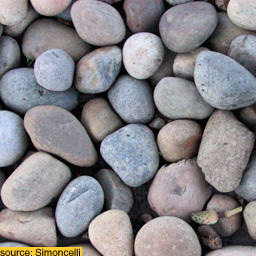
\includegraphics[width=\textwidth]{images/04-experiment01/pebbles/target.jpg}
        \end{subfigure}
        \hfill
        \begin{subfigure}{0.24\textwidth}
            \centering
            
\includegraphics[width=\textwidth]{images/04-experiment01/pebbles/white_bg.jpg}
        \end{subfigure}
        \hfill
        \begin{subfigure}{0.24\textwidth}
            \centering
            \begin{tikzpicture}
                \draw (0, 0) node[inner sep=0] {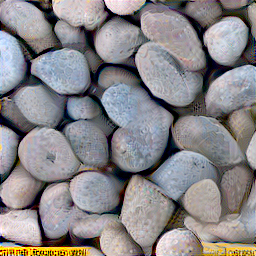
\includegraphics[width=\textwidth]{images/04-experiment01/pebbles/1000/white_im.jpg}};
                \fill[black] (-1.55, 1.0) rectangle ++(2.6, 0.6);
                \node [anchor=center] at (-0.25, 1.3) {{\color{white} Ours (Gatys)}};
            \end{tikzpicture}
        \end{subfigure}
        \hfill
        \begin{subfigure}{0.24\textwidth}
            \centering
            \begin{tikzpicture}
                \draw (0, 0) node[inner sep=0] {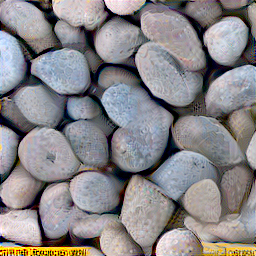
\includegraphics[width=\textwidth]{images/04-experiment01/pebbles/1000/white_proj.jpg}};
                \fill[black] (-1.55, 1.0) rectangle ++(2.6, 0.6);
                \node [anchor=center] at (-0.25, 1.3) {{\color{white} Ours (Gatys)}};
            \end{tikzpicture}
        \end{subfigure}

        \begin{subfigure}{0.24\textwidth}
            \centering
            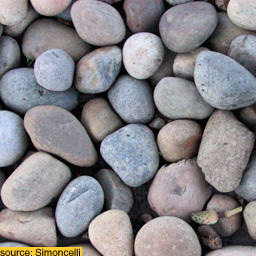
\includegraphics[width=\textwidth]{images/04-experiment01/pebbles/target.jpg}
        \end{subfigure}
        \hfill
        \begin{subfigure}{0.24\textwidth}
            \centering
            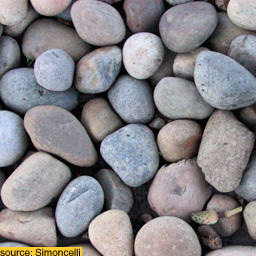
\includegraphics[width=\textwidth]{images/04-experiment01/pebbles/pebbles_bg.jpg}
        \end{subfigure}
        \hfill
        \begin{subfigure}{0.24\textwidth}
            \centering
            \begin{tikzpicture}
                \draw (0, 0) node[inner sep=0] {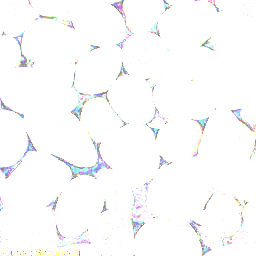
\includegraphics[width=\textwidth]{images/04-experiment01/pebbles/1000/pebbles_im.jpg}};
                \fill[black] (-1.55, 1.0) rectangle ++(2.6, 0.6);
                \node [anchor=center] at (-0.25, 1.3) {{\color{white} Ours (Gatys)}};
            \end{tikzpicture}
        \end{subfigure}
        \hfill
        \begin{subfigure}{0.24\textwidth}
            \centering
            \begin{tikzpicture}
                \draw (0, 0) node[inner sep=0] {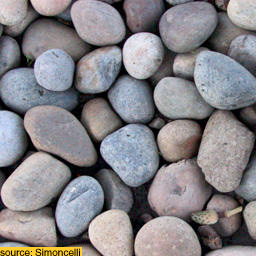
\includegraphics[width=\textwidth]{images/04-experiment01/pebbles/1000/pebbles_proj.jpg}};
                \fill[black] (-1.55, 1.0) rectangle ++(2.6, 0.6);
                \node [anchor=center] at (-0.25, 1.3) {{\color{white} Ours (Gatys)}};
            \end{tikzpicture}
        \end{subfigure}

        \begin{subfigure}{0.24\textwidth}
            \centering
            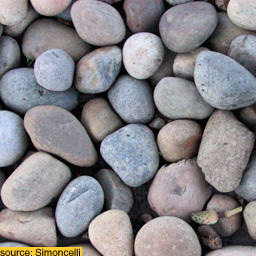
\includegraphics[width=\textwidth]{images/04-experiment01/pebbles/target.jpg}
        \end{subfigure}
        \hfill
        \begin{subfigure}{0.24\textwidth}
            \centering
            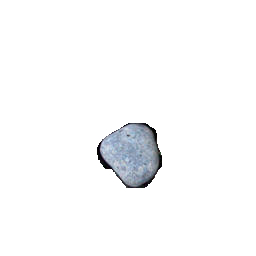
\includegraphics[width=\textwidth]{images/04-experiment01/pebbles/one_bg.jpg}
        \end{subfigure}
        \hfill
        \begin{subfigure}{0.24\textwidth}
            \centering
            \begin{tikzpicture}
                \draw (0, 0) node[inner sep=0] {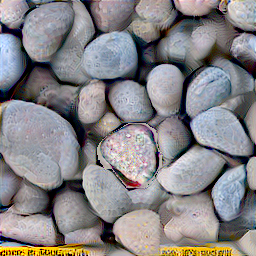
\includegraphics[width=\textwidth]{images/04-experiment01/pebbles/1000/one_im.jpg}};
                \fill[black] (-1.55, 1.0) rectangle ++(2.6, 0.6);
                \node [anchor=center] at (-0.25, 1.3) {{\color{white} Ours (Gatys)}};
            \end{tikzpicture}
        \end{subfigure}
        \hfill
        \begin{subfigure}{0.24\textwidth}
            \centering
            \begin{tikzpicture}
                \draw (0, 0) node[inner sep=0] {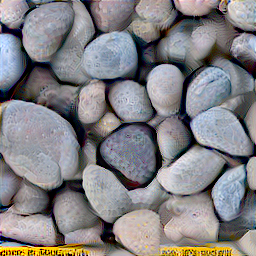
\includegraphics[width=\textwidth]{images/04-experiment01/pebbles/1000/one_proj.jpg}};
                \fill[black] (-1.55, 1.0) rectangle ++(2.6, 0.6);
                \node [anchor=center] at (-0.25, 1.3) {{\color{white} Ours (Gatys)}};
            \end{tikzpicture}
        \end{subfigure}

        \begin{subfigure}{0.24\textwidth}
            \centering
            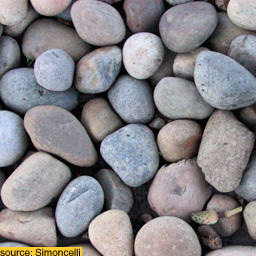
\includegraphics[width=\textwidth]{images/04-experiment01/pebbles/target.jpg}
        \end{subfigure}
        \hfill
        \begin{subfigure}{0.24\textwidth}
            \centering
            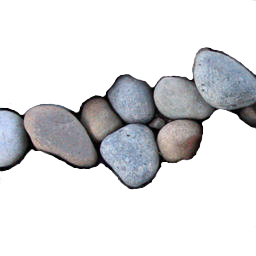
\includegraphics[width=\textwidth]{images/04-experiment01/pebbles/some_bg.jpg}
        \end{subfigure}
        \hfill
        \begin{subfigure}{0.24\textwidth}
            \centering
            \begin{tikzpicture}
                \draw (0, 0) node[inner sep=0] {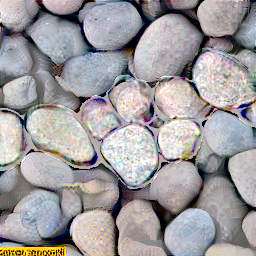
\includegraphics[width=\textwidth]{images/04-experiment01/pebbles/1000/some_im.jpg}};
                \fill[black] (-1.55, 1.0) rectangle ++(2.6, 0.6);
                \node [anchor=center] at (-0.25, 1.3) {{\color{white} Ours (Gatys)}};
            \end{tikzpicture}
        \end{subfigure}
        \hfill
        \begin{subfigure}{0.24\textwidth}
            \centering
            \begin{tikzpicture}
                \draw (0, 0) node[inner sep=0] {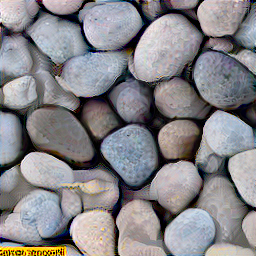
\includegraphics[width=\textwidth]{images/04-experiment01/pebbles/1000/some_proj.jpg}};
                \fill[black] (-1.55, 1.0) rectangle ++(2.6, 0.6);
                \node [anchor=center] at (-0.25, 1.3) {{\color{white} Ours (Gatys)}};
            \end{tikzpicture}
        \end{subfigure}
        
        \begin{subfigure}{0.24\textwidth}
            \centering
            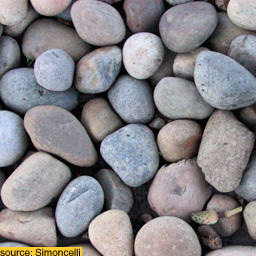
\includegraphics[width=\textwidth]{images/04-experiment01/pebbles/target.jpg}
            \caption*{Desired appearance \(\bm{y}\)}
        \end{subfigure}
        \hfill
        \begin{subfigure}{0.24\textwidth}
            \centering
            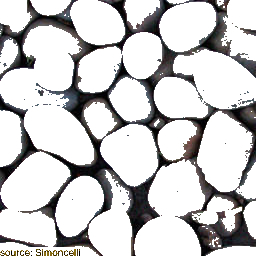
\includegraphics[width=\textwidth]{images/04-experiment01/pebbles/threshold_bg.jpg}
            \caption*{Background}
            \vspace*{5mm}
        \end{subfigure}
        \hfill
        \begin{subfigure}{0.24\textwidth}
            \centering
            \begin{tikzpicture}
                \draw (0, 0) node[inner sep=0] {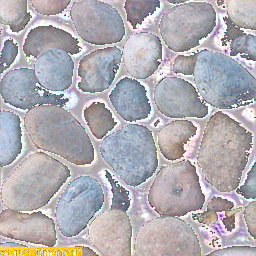
\includegraphics[width=\textwidth]{images/04-experiment01/pebbles/1000/threshold_im.jpg}};
                \fill[black] (-1.55, 1.0) rectangle ++(2.6, 0.6);
                \node [anchor=center] at (-0.25, 1.3) {{\color{white} Ours (Gatys)}};
            \end{tikzpicture}
            \caption*{Compensated projection image \(\bm{p}\)}
        \end{subfigure}
        \hfill
        \begin{subfigure}{0.24\textwidth}
            \centering
            \begin{tikzpicture}
                \draw (0, 0) node[inner sep=0] {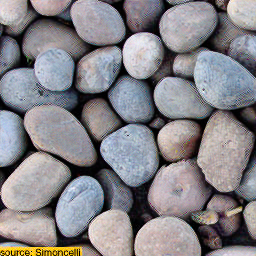
\includegraphics[width=\textwidth]{images/04-experiment01/pebbles/1000/threshold_proj.jpg}};
                \fill[black] (-1.55, 1.0) rectangle ++(2.6, 0.6);
                \node [anchor=center] at (-0.25, 1.3) {{\color{white} Ours (Gatys)}};
            \end{tikzpicture}
            \caption*{Final appearance \(r(\bm{p})\)}
        \end{subfigure}
    \end{subfigure}
    \caption{These results complement Section~\ref{section:results-experiments-01}. Texture source: \citet{Gatys2015}}
    \label{fig:ex01-complete-pebbles-1000steps}
\end{figure}

% EX01 - Flowers
\begin{figure}[]
    \centering    
    \begin{subfigure}{\textwidth}
        \centering
        \begin{subfigure}{0.24\textwidth}
            \centering
            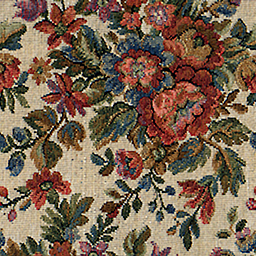
\includegraphics[width=\textwidth]{images/04-experiment01/flowers/target.jpg}
        \end{subfigure}
        \hfill
        \begin{subfigure}{0.24\textwidth}
            \centering
            
\includegraphics[width=\textwidth]{images/04-experiment01/flowers/white_bg.jpg}
        \end{subfigure}
        \hfill
        \begin{subfigure}{0.24\textwidth}
            \centering
            \begin{tikzpicture}
                \draw (0, 0) node[inner sep=0] {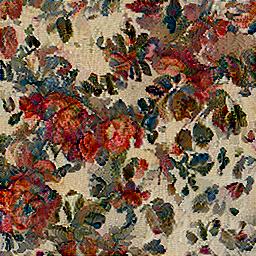
\includegraphics[width=\textwidth]{images/04-experiment01/flowers/1000/white_im.jpg}};
                \fill[black] (-1.55, 1.0) rectangle ++(2.6, 0.6);
                \node [anchor=center] at (-0.25, 1.3) {{\color{white} Ours (Gatys)}};
            \end{tikzpicture}
        \end{subfigure}
        \hfill
        \begin{subfigure}{0.24\textwidth}
            \centering
            \begin{tikzpicture}
                \draw (0, 0) node[inner sep=0] {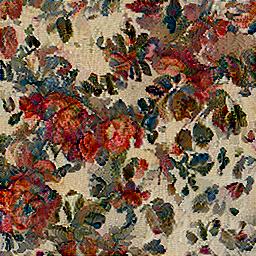
\includegraphics[width=\textwidth]{images/04-experiment01/flowers/1000/white_proj.jpg}};
                \fill[black] (-1.55, 1.0) rectangle ++(2.6, 0.6);
                \node [anchor=center] at (-0.25, 1.3) {{\color{white} Ours (Gatys)}};
            \end{tikzpicture}
        \end{subfigure}

        \begin{subfigure}{0.24\textwidth}
            \centering
            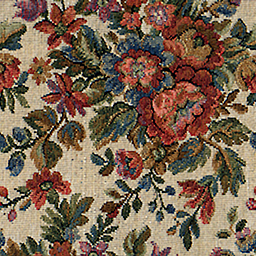
\includegraphics[width=\textwidth]{images/04-experiment01/flowers/target.jpg}
        \end{subfigure}
        \hfill
        \begin{subfigure}{0.24\textwidth}
            \centering
            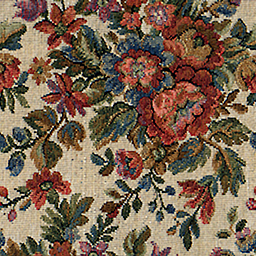
\includegraphics[width=\textwidth]{images/04-experiment01/flowers/flowers_bg.jpg}
        \end{subfigure}
        \hfill
        \begin{subfigure}{0.24\textwidth}
            \centering
            \begin{tikzpicture}
                \draw (0, 0) node[inner sep=0] {
\includegraphics[width=\textwidth]{images/04-experiment01/flowers/1000/flowers_im.jpg}};
                \fill[black] (-1.55, 1.0) rectangle ++(2.6, 0.6);
                \node [anchor=center] at (-0.25, 1.3) {{\color{white} Ours (Gatys)}};
            \end{tikzpicture}
        \end{subfigure}
        \hfill
        \begin{subfigure}{0.24\textwidth}
            \centering
            \begin{tikzpicture}
                \draw (0, 0) node[inner sep=0] {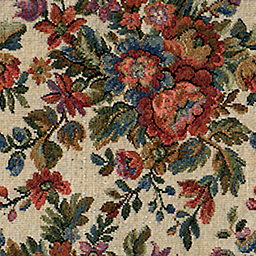
\includegraphics[width=\textwidth]{images/04-experiment01/flowers/1000/flowers_proj.jpg}};
                \fill[black] (-1.55, 1.0) rectangle ++(2.6, 0.6);
                \node [anchor=center] at (-0.25, 1.3) {{\color{white} Ours (Gatys)}};
            \end{tikzpicture}
        \end{subfigure}

        \begin{subfigure}{0.24\textwidth}
            \centering
            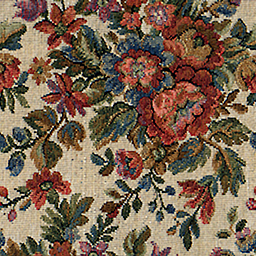
\includegraphics[width=\textwidth]{images/04-experiment01/flowers/target.jpg}
        \end{subfigure}
        \hfill
        \begin{subfigure}{0.24\textwidth}
            \centering
            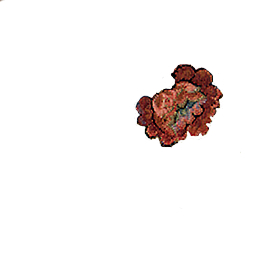
\includegraphics[width=\textwidth]{images/04-experiment01/flowers/one_bg.jpg}
        \end{subfigure}
        \hfill
        \begin{subfigure}{0.24\textwidth}
            \centering
            \begin{tikzpicture}
                \draw (0, 0) node[inner sep=0] {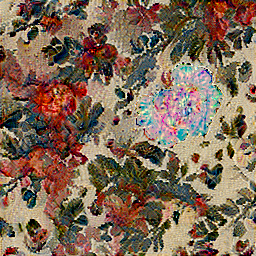
\includegraphics[width=\textwidth]{images/04-experiment01/flowers/1000/one_im.jpg}};
                \fill[black] (-1.55, 1.0) rectangle ++(2.6, 0.6);
                \node [anchor=center] at (-0.25, 1.3) {{\color{white} Ours (Gatys)}};
            \end{tikzpicture}
        \end{subfigure}
        \hfill
        \begin{subfigure}{0.24\textwidth}
            \centering
            \begin{tikzpicture}
                \draw (0, 0) node[inner sep=0] {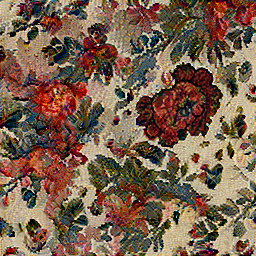
\includegraphics[width=\textwidth]{images/04-experiment01/flowers/1000/one_proj.jpg}};
                \fill[black] (-1.55, 1.0) rectangle ++(2.6, 0.6);
                \node [anchor=center] at (-0.25, 1.3) {{\color{white} Ours (Gatys)}};
            \end{tikzpicture}
        \end{subfigure}

        \begin{subfigure}{0.24\textwidth}
            \centering
            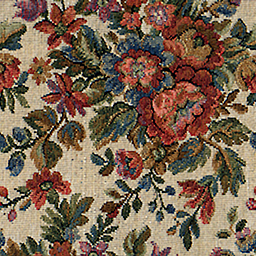
\includegraphics[width=\textwidth]{images/04-experiment01/flowers/target.jpg}
        \end{subfigure}
        \hfill
        \begin{subfigure}{0.24\textwidth}
            \centering
            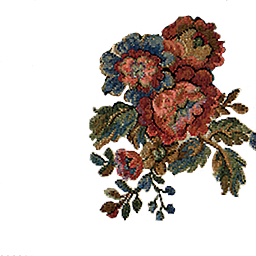
\includegraphics[width=\textwidth]{images/04-experiment01/flowers/some_bg.jpg}
        \end{subfigure}
        \hfill
        \begin{subfigure}{0.24\textwidth}
            \centering
            \begin{tikzpicture}
                \draw (0, 0) node[inner sep=0] {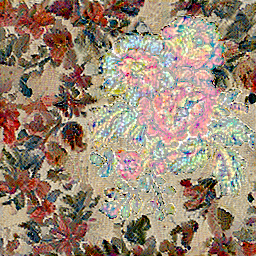
\includegraphics[width=\textwidth]{images/04-experiment01/flowers/1000/some_im.jpg}};
                \fill[black] (-1.55, 1.0) rectangle ++(2.6, 0.6);
                \node [anchor=center] at (-0.25, 1.3) {{\color{white} Ours (Gatys)}};
            \end{tikzpicture}
        \end{subfigure}
        \hfill
        \begin{subfigure}{0.24\textwidth}
            \centering
            \begin{tikzpicture}
                \draw (0, 0) node[inner sep=0] {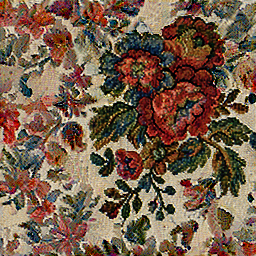
\includegraphics[width=\textwidth]{images/04-experiment01/flowers/1000/some_proj.jpg}};
                \fill[black] (-1.55, 1.0) rectangle ++(2.6, 0.6);
                \node [anchor=center] at (-0.25, 1.3) {{\color{white} Ours (Gatys)}};
            \end{tikzpicture}
        \end{subfigure}
        
        \begin{subfigure}{0.24\textwidth}
            \centering
            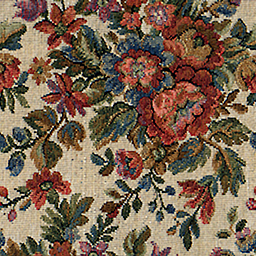
\includegraphics[width=\textwidth]{images/04-experiment01/flowers/target.jpg}
            \caption*{Desired appearance \(\bm{y}\)}
        \end{subfigure}
        \hfill
        \begin{subfigure}{0.24\textwidth}
            \centering
            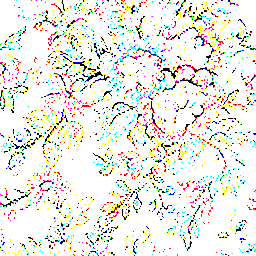
\includegraphics[width=\textwidth]{images/04-experiment01/flowers/threshold_bg.jpg}
            \caption*{Background}
            \vspace*{5mm}
        \end{subfigure}
        \hfill
        \begin{subfigure}{0.24\textwidth}
            \centering
            \begin{tikzpicture}
                \draw (0, 0) node[inner sep=0] {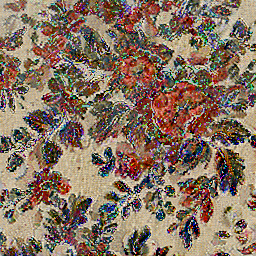
\includegraphics[width=\textwidth]{images/04-experiment01/flowers/1000/threshold_im.jpg}};
                \fill[black] (-1.55, 1.0) rectangle ++(2.6, 0.6);
                \node [anchor=center] at (-0.25, 1.3) {{\color{white} Ours (Gatys)}};
            \end{tikzpicture}
            \caption*{Compensated projection image \(\bm{p}\)}
        \end{subfigure}
        \hfill
        \begin{subfigure}{0.24\textwidth}
            \centering
            \begin{tikzpicture}
                \draw (0, 0) node[inner sep=0] {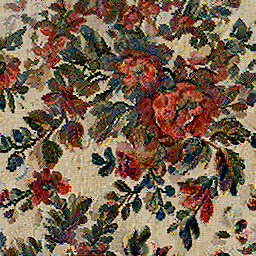
\includegraphics[width=\textwidth]{images/04-experiment01/flowers/1000/threshold_proj.jpg}};
                \fill[black] (-1.55, 1.0) rectangle ++(2.6, 0.6);
                \node [anchor=center] at (-0.25, 1.3) {{\color{white} Ours (Gatys)}};
            \end{tikzpicture}
            \caption*{Final appearance \(r(\bm{p})\)}
        \end{subfigure}
    \end{subfigure}
    \caption{These results complement Section~\ref{section:results-experiments-01}. Texture source: \citet{Pixar128}}
    \label{fig:ex01-complete-flowers-1000steps}
\end{figure}

% EX02 - Human - Marble, wood
\begin{figure}[]
    \centering    
    \begin{subfigure}{\textwidth}
        \centering
        \begin{subfigure}{0.2\textwidth}
            \centering
            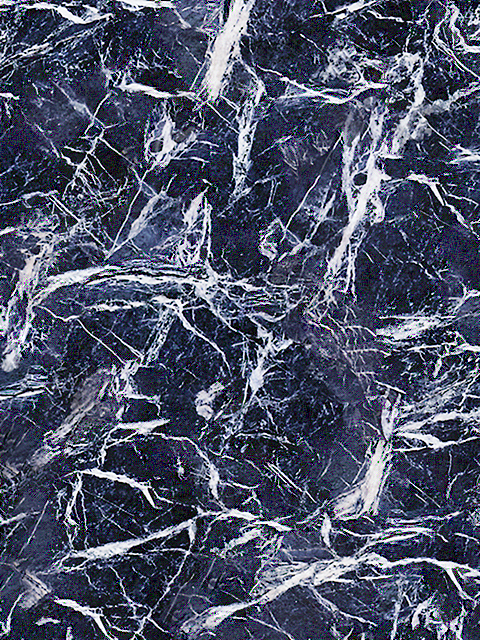
\includegraphics[width=\textwidth]{images/04-experiment02/human/marble/target.jpg}
            \caption*{Desired appearance \(\bm{y}\)}
        \end{subfigure}
        \hfill
        \begin{subfigure}{0.78\textwidth}
            \centering
            \begin{subfigure}{0.32\textwidth}
                \centering
                \begin{tikzpicture}
                    \draw (0, 0) node[inner sep=0] {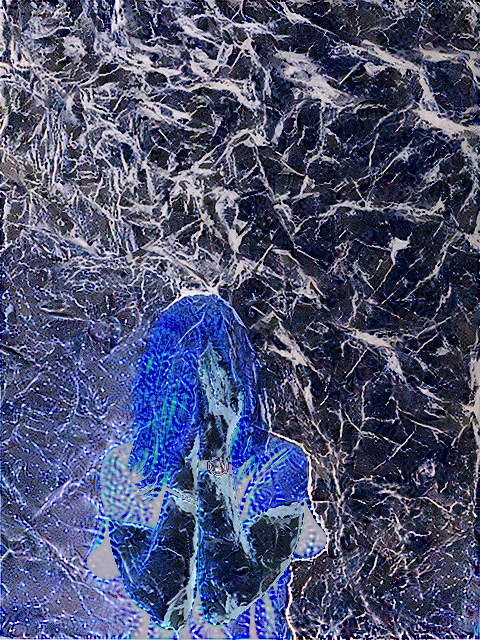
\includegraphics[width=\textwidth]{images/04-experiment02/human/marble/gatys_im.jpg}};
                    \fill[black] (-1.0, 1.6) rectangle ++(2.6, 0.6);
                    \node [anchor=center] at (0.3, 1.9) {{\color{white} Ours (Gatys)}};
                \end{tikzpicture}
            \end{subfigure}
            \hfill
            \begin{subfigure}{0.32\textwidth}
                \centering
                \begin{tikzpicture}
                    \draw (0, 0) node[inner sep=0] {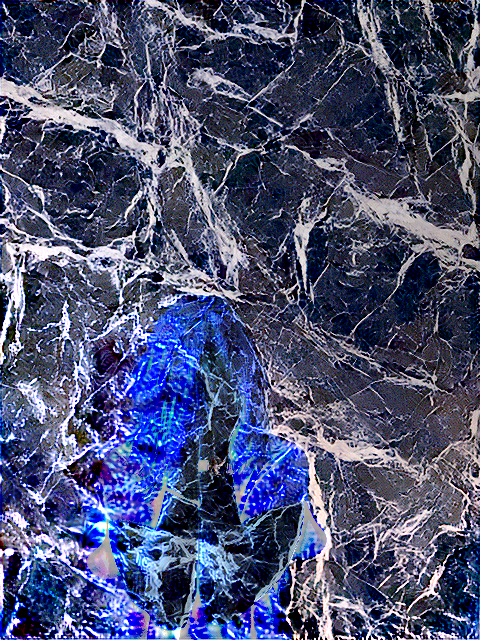
\includegraphics[width=\textwidth]{images/04-experiment02/human/marble/improved_im.jpg}};
                    \fill[black] (-1.5, 1.6) rectangle ++(3.1, 0.6);
                    \node [anchor=center] at (0.05, 1.9) {{\color{white} \small{Ours (Improved)}}};
                \end{tikzpicture}
            \end{subfigure}
            \hfill
            \begin{subfigure}{0.32\textwidth}
                \centering
                \begin{tikzpicture}
                    \draw (0, 0) node[inner sep=0] {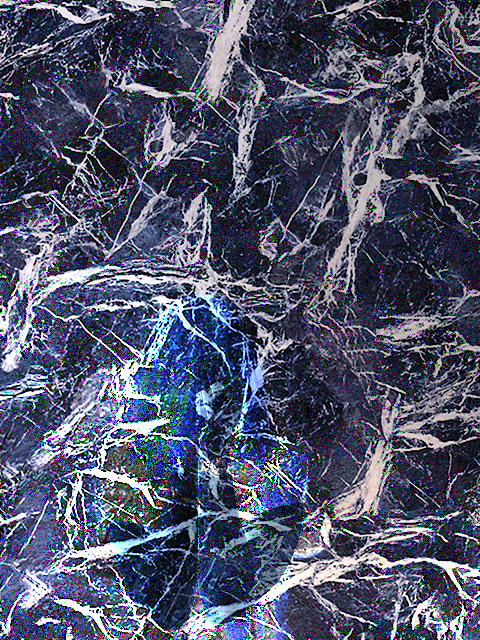
\includegraphics[width=\textwidth]{images/04-experiment02/human/marble/pixel_im.jpg}};
                    \fill[black] (-1.0, 1.6) rectangle ++(2.6, 0.6);
                    \node [anchor=center] at (0.3, 1.9) {{\color{white} Baseline}};
                \end{tikzpicture}
            \end{subfigure}
            \caption*{Compensated projection image \(\bm{p}\)}
        \end{subfigure}
        
        \begin{subfigure}{0.2\textwidth}
            \centering
            
\includegraphics[width=\textwidth]{images/04-experiment02/human/bg.jpg}
            \caption*{Background}
        \end{subfigure}
        \hfill
        \begin{subfigure}{0.78\textwidth}
            \begin{subfigure}{0.32\textwidth}
                \centering
                \begin{tikzpicture}
                    \draw (0, 0) node[inner sep=0] {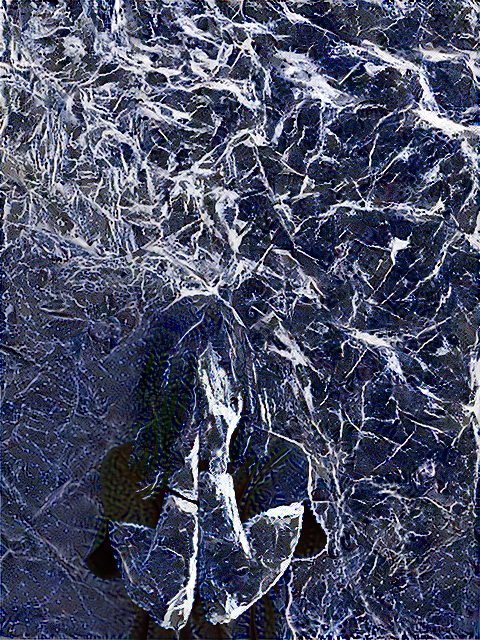
\includegraphics[width=\textwidth]{images/04-experiment02/human/marble/gatys_proj.jpg}};
                    \fill[black] (-1.0, 1.6) rectangle ++(2.6, 0.6);
                    \node [anchor=center] at (0.3, 1.9) {{\color{white} Ours (Gatys)}};
                \end{tikzpicture}
            \end{subfigure}
            \hfill
            \begin{subfigure}{0.32\textwidth}
                \centering
                \begin{tikzpicture}
                    \draw (0, 0) node[inner sep=0] {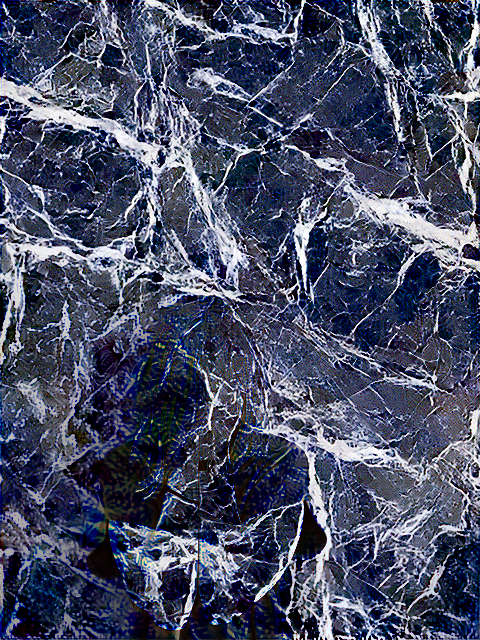
\includegraphics[width=\textwidth]{images/04-experiment02/human/marble/improved_proj.jpg}};
                    \fill[black] (-1.5, 1.6) rectangle ++(3.1, 0.6);
                    \node [anchor=center] at (0.05, 1.9) {{\color{white} \small{Ours (Improved)}}};
                \end{tikzpicture}
            \end{subfigure}
            \hfill
            \begin{subfigure}{0.32\textwidth}
                \centering
                \begin{tikzpicture}
                    \draw (0, 0) node[inner sep=0] {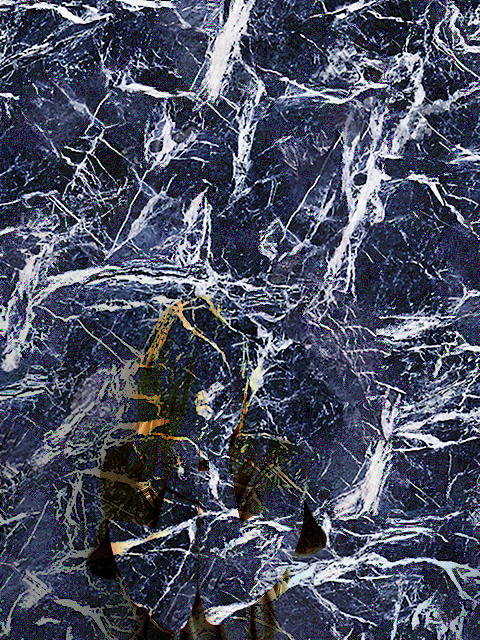
\includegraphics[width=\textwidth]{images/04-experiment02/human/marble/pixel_proj.jpg}};
                    \fill[black] (-1.0, 1.6) rectangle ++(2.6, 0.6);
                    \node [anchor=center] at (0.3, 1.9) {{\color{white} Baseline}};
                \end{tikzpicture}
            \end{subfigure}
            \caption*{Final appearance \(r(\bm{p})\)}
        \end{subfigure}
    \end{subfigure}

    \begin{subfigure}{\textwidth}
        \centering
        \begin{subfigure}{0.2\textwidth}
            \centering
            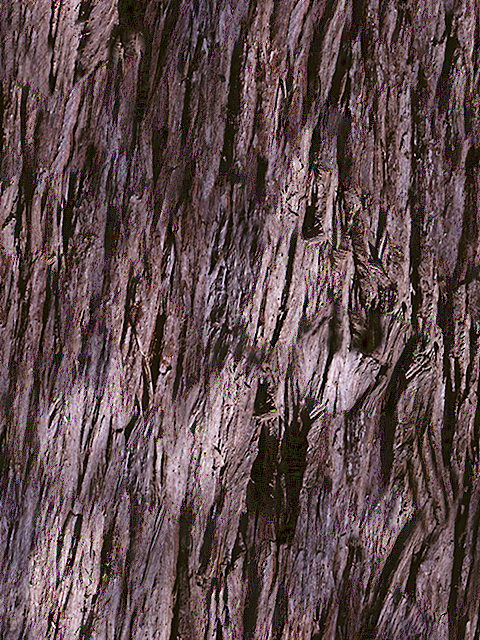
\includegraphics[width=\textwidth]{images/04-experiment02/human/wood/target.jpg}
            \caption*{Desired appearance \(\bm{y}\)}
        \end{subfigure}
        \hfill
        \begin{subfigure}{0.78\textwidth}
            \centering
            \begin{subfigure}{0.32\textwidth}
                \centering
                \begin{tikzpicture}
                    \draw (0, 0) node[inner sep=0] {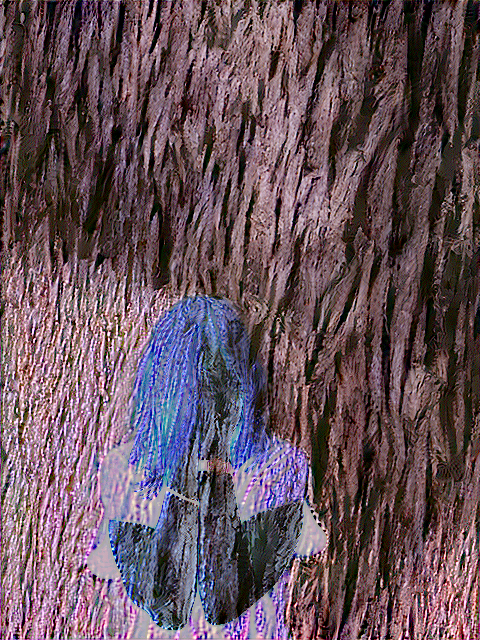
\includegraphics[width=\textwidth]{images/04-experiment02/human/wood/gatys_im.jpg}};
                    \fill[black] (-1.0, 1.6) rectangle ++(2.6, 0.6);
                    \node [anchor=center] at (0.3, 1.9) {{\color{white} Ours (Gatys)}};
                \end{tikzpicture}
            \end{subfigure}
            \hfill
            \begin{subfigure}{0.32\textwidth}
                \centering
                \begin{tikzpicture}
                    \draw (0, 0) node[inner sep=0] {\includegraphics[width=\textwidth]{images/04-experiment02/human/wood/improved_im.jpg}};
                    \fill[black] (-1.5, 1.6) rectangle ++(3.1, 0.6);
                    \node [anchor=center] at (0.05, 1.9) {{\color{white} \small{Ours (Improved)}}};
                \end{tikzpicture}
            \end{subfigure}
            \hfill
            \begin{subfigure}{0.32\textwidth}
                \centering
                \begin{tikzpicture}
                    \draw (0, 0) node[inner sep=0] {\includegraphics[width=\textwidth]{images/04-experiment02/human/wood/pixel_im.jpg}};
                    \fill[black] (-1.0, 1.6) rectangle ++(2.6, 0.6);
                    \node [anchor=center] at (0.3, 1.9) {{\color{white} Baseline}};
                \end{tikzpicture}
            \end{subfigure}
            \caption*{Compensated projection image \(\bm{p}\)}
        \end{subfigure}
        
        \begin{subfigure}{0.2\textwidth}
            \centering
            \includegraphics[width=\textwidth]{images/04-experiment02/human/bg.jpg}
            \caption*{Background}
        \end{subfigure}
        \hfill
        \begin{subfigure}{0.78\textwidth}
            \centering
            \begin{subfigure}{0.32\textwidth}
                \centering
                \begin{tikzpicture}
                    \draw (0, 0) node[inner sep=0] {\includegraphics[width=\textwidth]{images/04-experiment02/human/wood/gatys_proj.jpg}};
                    \fill[black] (-1.0, 1.6) rectangle ++(2.6, 0.6);
                    \node [anchor=center] at (0.3, 1.9) {{\color{white} Ours (Gatys)}};
                \end{tikzpicture}
            \end{subfigure}
            \hfill
            \begin{subfigure}{0.32\textwidth}
                \centering
                \begin{tikzpicture}
                    \draw (0, 0) node[inner sep=0] {\includegraphics[width=\textwidth]{images/04-experiment02/human/wood/improved_proj.jpg}};
                    \fill[black] (-1.5, 1.6) rectangle ++(3.1, 0.6);
                    \node [anchor=center] at (0.05, 1.9) {{\color{white} \small{Ours (Improved)}}};
                \end{tikzpicture}
            \end{subfigure}
            \hfill
            \begin{subfigure}{0.32\textwidth}
                \centering
                \begin{tikzpicture}
                    \draw (0, 0) node[inner sep=0] {\includegraphics[width=\textwidth]{images/04-experiment02/human/wood/pixel_proj.jpg}};
                    \fill[black] (-1.0, 1.6) rectangle ++(2.6, 0.6);
                    \node [anchor=center] at (0.3, 1.9) {{\color{white} Baseline}};
                \end{tikzpicture}
            \end{subfigure}
            \caption*{Final appearance \(r(\bm{p})\)}
        \end{subfigure}
    \end{subfigure}
    \caption{These results complement Section~\ref{section:results-experiments-02}. Texture source: \citet{Pixar128}}
    \label{fig:ex02-complete-human-marble_wood}
\end{figure}

% EX02 - Human - Flowers, flowers2
\begin{figure}[]
    \centering    
    \begin{subfigure}{\textwidth}
        \centering
        \begin{subfigure}{0.2\textwidth}
            \centering
            \includegraphics[width=\textwidth]{images/04-experiment02/human/flowers/target.jpg}
            \caption*{Desired appearance \(\bm{y}\)}
        \end{subfigure}
        \hfill
        \begin{subfigure}{0.78\textwidth}
            \centering
            \begin{subfigure}{0.32\textwidth}
                \centering
                \begin{tikzpicture}
                    \draw (0, 0) node[inner sep=0] {\includegraphics[width=\textwidth]{images/04-experiment02/human/flowers/gatys_im.jpg}};
                    \fill[black] (-1.0, 1.6) rectangle ++(2.6, 0.6);
                    \node [anchor=center] at (0.3, 1.9) {{\color{white} Ours (Gatys)}};
                \end{tikzpicture}
            \end{subfigure}
            \hfill
            \begin{subfigure}{0.32\textwidth}
                \centering
                \begin{tikzpicture}
                    \draw (0, 0) node[inner sep=0] {\includegraphics[width=\textwidth]{images/04-experiment02/human/flowers/improved_im.jpg}};
                    \fill[black] (-1.5, 1.6) rectangle ++(3.1, 0.6);
                    \node [anchor=center] at (0.05, 1.9) {{\color{white} \small{Ours (Improved)}}};
                \end{tikzpicture}
            \end{subfigure}
            \hfill
            \begin{subfigure}{0.32\textwidth}
                \centering
                \begin{tikzpicture}
                    \draw (0, 0) node[inner sep=0] {\includegraphics[width=\textwidth]{images/04-experiment02/human/flowers/pixel_im.jpg}};
                    \fill[black] (-1.0, 1.6) rectangle ++(2.6, 0.6);
                    \node [anchor=center] at (0.3, 1.9) {{\color{white} Baseline}};
                \end{tikzpicture}
            \end{subfigure}
            \caption*{Compensated projection image \(\bm{p}\)}
        \end{subfigure}
        
        \begin{subfigure}{0.2\textwidth}
            \centering
            \includegraphics[width=\textwidth]{images/04-experiment02/human/bg.jpg}
            \caption*{Background}
        \end{subfigure}
        \hfill
        \begin{subfigure}{0.78\textwidth}
            \centering
            \begin{subfigure}{0.32\textwidth}
                \centering
                \begin{tikzpicture}
                    \draw (0, 0) node[inner sep=0] {\includegraphics[width=\textwidth]{images/04-experiment02/human/flowers/gatys_proj.jpg}};
                    \fill[black] (-1.0, 1.6) rectangle ++(2.6, 0.6);
                    \node [anchor=center] at (0.3, 1.9) {{\color{white} Ours (Gatys)}};
                \end{tikzpicture}
            \end{subfigure}
            \hfill
            \begin{subfigure}{0.32\textwidth}
                \centering
                \begin{tikzpicture}
                    \draw (0, 0) node[inner sep=0] {\includegraphics[width=\textwidth]{images/04-experiment02/human/flowers/improved_proj.jpg}};
                    \fill[black] (-1.5, 1.6) rectangle ++(3.1, 0.6);
                    \node [anchor=center] at (0.05, 1.9) {{\color{white} \small{Ours (Improved)}}};
                \end{tikzpicture}
            \end{subfigure}
            \hfill
            \begin{subfigure}{0.32\textwidth}
                \centering
                \begin{tikzpicture}
                    \draw (0, 0) node[inner sep=0] {\includegraphics[width=\textwidth]{images/04-experiment02/human/flowers/pixel_proj.jpg}};
                    \fill[black] (-1.0, 1.6) rectangle ++(2.6, 0.6);
                    \node [anchor=center] at (0.3, 1.9) {{\color{white} Baseline}};
                \end{tikzpicture}
            \end{subfigure}
            \caption*{Final appearance \(r(\bm{p})\)}
        \end{subfigure}
    \end{subfigure}

    \begin{subfigure}{\textwidth}
        \centering
        \begin{subfigure}{0.2\textwidth}
            \centering
            \includegraphics[width=\textwidth]{images/04-experiment02/human/flowers2/target.jpg}
            \caption*{Desired appearance \(\bm{y}\)}
        \end{subfigure}
        \hfill
        \begin{subfigure}{0.78\textwidth}
            \centering
            \begin{subfigure}{0.32\textwidth}
                \centering
                \begin{tikzpicture}
                    \draw (0, 0) node[inner sep=0] {\includegraphics[width=\textwidth]{images/04-experiment02/human/flowers2/gatys_im.jpg}};
                    \fill[black] (-1.0, 1.6) rectangle ++(2.6, 0.6);
                    \node [anchor=center] at (0.3, 1.9) {{\color{white} Ours (Gatys)}};
                \end{tikzpicture}
            \end{subfigure}
            \hfill
            \begin{subfigure}{0.32\textwidth}
                \centering
                \begin{tikzpicture}
                    \draw (0, 0) node[inner sep=0] {\includegraphics[width=\textwidth]{images/04-experiment02/human/flowers2/improved_im.jpg}};
                    \fill[black] (-1.5, 1.6) rectangle ++(3.1, 0.6);
                    \node [anchor=center] at (0.05, 1.9) {{\color{white} \small{Ours (Improved)}}};
                \end{tikzpicture}
            \end{subfigure}
            \hfill
            \begin{subfigure}{0.32\textwidth}
                \centering
                \begin{tikzpicture}
                    \draw (0, 0) node[inner sep=0] {\includegraphics[width=\textwidth]{images/04-experiment02/human/flowers2/pixel_im.jpg}};
                    \fill[black] (-1.0, 1.6) rectangle ++(2.6, 0.6);
                    \node [anchor=center] at (0.3, 1.9) {{\color{white} Baseline}};
                \end{tikzpicture}
            \end{subfigure}
            \caption*{Compensated projection image \(\bm{p}\)}
        \end{subfigure}
        
        \begin{subfigure}{0.2\textwidth}
            \centering
            \includegraphics[width=\textwidth]{images/04-experiment02/human/bg.jpg}
            \caption*{Background}
        \end{subfigure}
        \hfill
        \begin{subfigure}{0.78\textwidth}
            \centering
            \begin{subfigure}{0.32\textwidth}
                \centering
                \begin{tikzpicture}
                    \draw (0, 0) node[inner sep=0] {\includegraphics[width=\textwidth]{images/04-experiment02/human/flowers2/gatys_proj.jpg}};
                    \fill[black] (-1.0, 1.6) rectangle ++(2.6, 0.6);
                    \node [anchor=center] at (0.3, 1.9) {{\color{white} Ours (Gatys)}};
                \end{tikzpicture}
            \end{subfigure}
            \hfill
            \begin{subfigure}{0.32\textwidth}
                \centering
                \begin{tikzpicture}
                    \draw (0, 0) node[inner sep=0] {\includegraphics[width=\textwidth]{images/04-experiment02/human/flowers2/improved_proj.jpg}};
                    \fill[black] (-1.5, 1.6) rectangle ++(3.1, 0.6);
                    \node [anchor=center] at (0.05, 1.9) {{\color{white} \small{Ours (Improved)}}};
                \end{tikzpicture}
            \end{subfigure}
            \hfill
            \begin{subfigure}{0.32\textwidth}
                \centering
                \begin{tikzpicture}
                    \draw (0, 0) node[inner sep=0] {\includegraphics[width=\textwidth]{images/04-experiment02/human/flowers2/pixel_proj.jpg}};
                    \fill[black] (-1.0, 1.6) rectangle ++(2.6, 0.6);
                    \node [anchor=center] at (0.3, 1.9) {{\color{white} Baseline}};
                \end{tikzpicture}
            \end{subfigure}
            \caption*{Final appearance \(r(\bm{p})\)}
        \end{subfigure}
    \end{subfigure}
    \caption{These results complement Section~\ref{section:results-experiments-02}. Texture source: \citet{Pixar128}}
    \label{fig:ex02-complete-human-flowers_flowers2}
\end{figure}

% EX02 - Human - Pebbles
\begin{figure}[]
    \centering    
    \begin{subfigure}{\textwidth}
        \centering
        \begin{subfigure}{0.2\textwidth}
            \centering
            \includegraphics[width=\textwidth]{images/04-experiment02/human/pebbles/target.jpg}
            \caption*{Desired appearance \(\bm{y}\)}
        \end{subfigure}
        \hfill
        \begin{subfigure}{0.78\textwidth}
            \centering
            \begin{subfigure}{0.32\textwidth}
                \centering
                \begin{tikzpicture}
                    \draw (0, 0) node[inner sep=0] {\includegraphics[width=\textwidth]{images/04-experiment02/human/pebbles/gatys_im.jpg}};
                    \fill[black] (-1.0, 1.6) rectangle ++(2.6, 0.6);
                    \node [anchor=center] at (0.3, 1.9) {{\color{white} Ours (Gatys)}};
                \end{tikzpicture}
            \end{subfigure}
            \hfill
            \begin{subfigure}{0.32\textwidth}
                \centering
                \begin{tikzpicture}
                    \draw (0, 0) node[inner sep=0] {\includegraphics[width=\textwidth]{images/04-experiment02/human/pebbles/improved_im.jpg}};
                    \fill[black] (-1.5, 1.6) rectangle ++(3.1, 0.6);
                    \node [anchor=center] at (0.05, 1.9) {{\color{white} \small{Ours (Improved)}}};
                \end{tikzpicture}
            \end{subfigure}
            \hfill
            \begin{subfigure}{0.32\textwidth}
                \centering
                \begin{tikzpicture}
                    \draw (0, 0) node[inner sep=0] {\includegraphics[width=\textwidth]{images/04-experiment02/human/pebbles/pixel_im.jpg}};
                    \fill[black] (-1.0, 1.6) rectangle ++(2.6, 0.6);
                    \node [anchor=center] at (0.3, 1.9) {{\color{white} Baseline}};
                \end{tikzpicture}
            \end{subfigure}
            \caption*{Compensated projection image \(\bm{p}\)}
        \end{subfigure}
        
        \begin{subfigure}{0.2\textwidth}
            \centering
            \includegraphics[width=\textwidth]{images/04-experiment02/human/bg.jpg}
            \caption*{Background}
        \end{subfigure}
        \hfill
        \begin{subfigure}{0.78\textwidth}
            \centering
            \begin{subfigure}{0.32\textwidth}
                \centering
                \begin{tikzpicture}
                    \draw (0, 0) node[inner sep=0] {\includegraphics[width=\textwidth]{images/04-experiment02/human/pebbles/gatys_proj.jpg}};
                    \fill[black] (-1.0, 1.6) rectangle ++(2.6, 0.6);
                    \node [anchor=center] at (0.3, 1.9) {{\color{white} Ours (Gatys)}};
                \end{tikzpicture}
            \end{subfigure}
            \hfill
            \begin{subfigure}{0.32\textwidth}
                \centering
                \begin{tikzpicture}
                    \draw (0, 0) node[inner sep=0] {\includegraphics[width=\textwidth]{images/04-experiment02/human/pebbles/improved_proj.jpg}};
                    \fill[black] (-1.5, 1.6) rectangle ++(3.1, 0.6);
                    \node [anchor=center] at (0.05, 1.9) {{\color{white} \small{Ours (Improved)}}};
                \end{tikzpicture}
            \end{subfigure}
            \hfill
            \begin{subfigure}{0.32\textwidth}
                \centering
                \begin{tikzpicture}
                    \draw (0, 0) node[inner sep=0] {\includegraphics[width=\textwidth]{images/04-experiment02/human/pebbles/pixel_proj.jpg}};
                    \fill[black] (-1.0, 1.6) rectangle ++(2.6, 0.6);
                    \node [anchor=center] at (0.3, 1.9) {{\color{white} Baseline}};
                \end{tikzpicture}
            \end{subfigure}
            \caption*{Final appearance \(r(\bm{p})\)}
        \end{subfigure}
    \end{subfigure}
    \caption{These results complement Section~\ref{section:results-experiments-02}. Texture source: \citet{Pixar128}}
    \label{fig:ex02-complete-human-pebbles}
\end{figure}

% EX02 - Carpet - Marble, wood, pebbles
\begin{figure}[]
    \centering    
    \begin{subfigure}{\textwidth}
        \centering
        \begin{subfigure}{0.2\textwidth}
            \centering
            \includegraphics[width=\textwidth]{images/04-experiment02/carpet/marble/target.jpg}
            \caption*{Desired appearance \(\bm{y}\)}
        \end{subfigure}
        \hfill
        \begin{subfigure}{0.78\textwidth}
            \centering
            \begin{subfigure}{0.32\textwidth}
                \centering
                \begin{tikzpicture}
                    \draw (0, 0) node[inner sep=0] {\includegraphics[width=\textwidth]{images/04-experiment02/carpet/marble/gatys_im.jpg}};
                    \fill[black] (-1.6, -1.2) rectangle ++(2.4, 0.5);
                    \node [anchor=center] at (-0.4, -0.95) {{\color{white} \small{Ours (Gatys)}}};
                \end{tikzpicture}
            \end{subfigure}
            \hfill
            \begin{subfigure}{0.32\textwidth}
                \centering
                \begin{tikzpicture}
                    \draw (0, 0) node[inner sep=0] {\includegraphics[width=\textwidth]{images/04-experiment02/carpet/marble/improved_im.jpg}};
                    \fill[black] (-1.6, -1.2) rectangle ++(2.75, 0.5);
                    \node [anchor=center] at (-0.225, -0.95) {{\color{white} \footnotesize{Ours (Improved)}}};
                \end{tikzpicture}
            \end{subfigure}
            \hfill
            \begin{subfigure}{0.32\textwidth}
                \centering
                \begin{tikzpicture}
                    \draw (0, 0) node[inner sep=0] {\includegraphics[width=\textwidth]{images/04-experiment02/carpet/marble/pixel_im.jpg}};
                    \fill[black] (-1.6, -1.2) rectangle ++(2.4, 0.5);
                    \node [anchor=center] at (-0.4, -0.95) {{\color{white} \small{Baseline}}};
                \end{tikzpicture}
            \end{subfigure}
            \caption*{Compensated projection image \(\bm{p}\)}
        \end{subfigure}
        
        \begin{subfigure}{0.2\textwidth}
            \centering
            \includegraphics[width=\textwidth]{images/04-experiment02/carpet/bg.jpg}
            \caption*{Background}
        \end{subfigure}
        \hfill
        \begin{subfigure}{0.78\textwidth}
            \centering
            \begin{subfigure}{0.32\textwidth}
                \centering
                \begin{tikzpicture}
                    \draw (0, 0) node[inner sep=0] {\includegraphics[width=\textwidth]{images/04-experiment02/carpet/marble/gatys_proj.jpg}};
                    \fill[black] (-1.6, -1.2) rectangle ++(2.4, 0.5);
                    \node [anchor=center] at (-0.4, -0.95) {{\color{white} \small{Ours (Gatys)}}};
                \end{tikzpicture}
            \end{subfigure}
            \hfill
            \begin{subfigure}{0.32\textwidth}
                \centering
                \begin{tikzpicture}
                    \draw (0, 0) node[inner sep=0] {\includegraphics[width=\textwidth]{images/04-experiment02/carpet/marble/improved_proj.jpg}};
                    \fill[black] (-1.6, -1.2) rectangle ++(2.75, 0.5);
                    \node [anchor=center] at (-0.225, -0.95) {{\color{white} \footnotesize{Ours (Improved)}}};
                \end{tikzpicture}
            \end{subfigure}
            \hfill
            \begin{subfigure}{0.32\textwidth}
                \centering
                \begin{tikzpicture}
                    \draw (0, 0) node[inner sep=0] {\includegraphics[width=\textwidth]{images/04-experiment02/carpet/marble/pixel_proj.jpg}};
                    \fill[black] (-1.6, -1.2) rectangle ++(2.4, 0.5);
                    \node [anchor=center] at (-0.4, -0.95) {{\color{white} \small{Baseline}}};
                \end{tikzpicture}
            \end{subfigure}
            \caption*{Final appearance \(r(\bm{p})\)}
        \end{subfigure}
    \end{subfigure}

    \begin{subfigure}{\textwidth}
        \centering
        \begin{subfigure}{0.2\textwidth}
            \centering
            \includegraphics[width=\textwidth]{images/04-experiment02/carpet/wood/target.jpg}
            \caption*{Desired appearance \(\bm{y}\)}
        \end{subfigure}
        \hfill
        \begin{subfigure}{0.78\textwidth}
            \centering
            \begin{subfigure}{0.32\textwidth}
                \centering
                \begin{tikzpicture}
                    \draw (0, 0) node[inner sep=0] {\includegraphics[width=\textwidth]{images/04-experiment02/carpet/wood/gatys_im.jpg}};
                    \fill[black] (-1.6, -1.2) rectangle ++(2.4, 0.5);
                    \node [anchor=center] at (-0.4, -0.95) {{\color{white} \small{Ours (Gatys)}}};
                \end{tikzpicture}
            \end{subfigure}
            \hfill
            \begin{subfigure}{0.32\textwidth}
                \centering
                \begin{tikzpicture}
                    \draw (0, 0) node[inner sep=0] {\includegraphics[width=\textwidth]{images/04-experiment02/carpet/wood/improved_im.jpg}};
                    \fill[black] (-1.6, -1.2) rectangle ++(2.75, 0.5);
                    \node [anchor=center] at (-0.225, -0.95) {{\color{white} \footnotesize{Ours (Improved)}}};
                \end{tikzpicture}
            \end{subfigure}
            \hfill
            \begin{subfigure}{0.32\textwidth}
                \centering
                \begin{tikzpicture}
                    \draw (0, 0) node[inner sep=0] {\includegraphics[width=\textwidth]{images/04-experiment02/carpet/wood/pixel_im.jpg}};
                    \fill[black] (-1.6, -1.2) rectangle ++(2.4, 0.5);
                    \node [anchor=center] at (-0.4, -0.95) {{\color{white} \small{Baseline}}};
                \end{tikzpicture}
            \end{subfigure}
            \caption*{Compensated projection image \(\bm{p}\)}
        \end{subfigure}
        
        \begin{subfigure}{0.2\textwidth}
            \centering
            \includegraphics[width=\textwidth]{images/04-experiment02/carpet/bg.jpg}
            \caption*{Background}
        \end{subfigure}
        \hfill
        \begin{subfigure}{0.78\textwidth}
            \centering
            \begin{subfigure}{0.32\textwidth}
                \centering
                \begin{tikzpicture}
                    \draw (0, 0) node[inner sep=0] {\includegraphics[width=\textwidth]{images/04-experiment02/carpet/wood/gatys_proj.jpg}};
                    \fill[black] (-1.6, -1.2) rectangle ++(2.4, 0.5);
                    \node [anchor=center] at (-0.4, -0.95) {{\color{white} \small{Ours (Gatys)}}};
                \end{tikzpicture}
            \end{subfigure}
            \hfill
            \begin{subfigure}{0.32\textwidth}
                \centering
                \begin{tikzpicture}
                    \draw (0, 0) node[inner sep=0] {\includegraphics[width=\textwidth]{images/04-experiment02/carpet/wood/improved_proj.jpg}};
                    \fill[black] (-1.6, -1.2) rectangle ++(2.75, 0.5);
                    \node [anchor=center] at (-0.225, -0.95) {{\color{white} \footnotesize{Ours (Improved)}}};
                \end{tikzpicture}
            \end{subfigure}
            \hfill
            \begin{subfigure}{0.32\textwidth}
                \centering
                \begin{tikzpicture}
                    \draw (0, 0) node[inner sep=0] {\includegraphics[width=\textwidth]{images/04-experiment02/carpet/wood/pixel_proj.jpg}};
                    \fill[black] (-1.6, -1.2) rectangle ++(2.4, 0.5);
                    \node [anchor=center] at (-0.4, -0.95) {{\color{white} \small{Baseline}}};
                \end{tikzpicture}
            \end{subfigure}
            \caption*{Final appearance \(r(\bm{p})\)}
        \end{subfigure}

        \begin{subfigure}{0.2\textwidth}
            \centering
            \includegraphics[width=\textwidth]{images/04-experiment02/carpet/pebbles/target.jpg}
            \caption*{Desired appearance \(\bm{y}\)}
        \end{subfigure}
        \hfill
        \begin{subfigure}{0.78\textwidth}
            \centering
            \begin{subfigure}{0.32\textwidth}
                \centering
                \begin{tikzpicture}
                    \draw (0, 0) node[inner sep=0] {\includegraphics[width=\textwidth]{images/04-experiment02/carpet/pebbles/gatys_im.jpg}};
                    \fill[black] (-1.6, -1.2) rectangle ++(2.4, 0.5);
                    \node [anchor=center] at (-0.4, -0.95) {{\color{white} \small{Ours (Gatys)}}};
                \end{tikzpicture}
            \end{subfigure}
            \hfill
            \begin{subfigure}{0.32\textwidth}
                \centering
                \begin{tikzpicture}
                    \draw (0, 0) node[inner sep=0] {\includegraphics[width=\textwidth]{images/04-experiment02/carpet/pebbles/improved_im.jpg}};
                    \fill[black] (-1.6, -1.2) rectangle ++(2.75, 0.5);
                    \node [anchor=center] at (-0.225, -0.95) {{\color{white} \footnotesize{Ours (Improved)}}};
                \end{tikzpicture}
            \end{subfigure}
            \hfill
            \begin{subfigure}{0.32\textwidth}
                \centering
                \begin{tikzpicture}
                    \draw (0, 0) node[inner sep=0] {\includegraphics[width=\textwidth]{images/04-experiment02/carpet/pebbles/pixel_im.jpg}};
                    \fill[black] (-1.6, -1.2) rectangle ++(2.4, 0.5);
                    \node [anchor=center] at (-0.4, -0.95) {{\color{white} \small{Baseline}}};
                \end{tikzpicture}
            \end{subfigure}
            \caption*{Compensated projection image \(\bm{p}\)}
        \end{subfigure}
        
        \begin{subfigure}{0.2\textwidth}
            \centering
            \includegraphics[width=\textwidth]{images/04-experiment02/carpet/bg.jpg}
            \caption*{Background}
        \end{subfigure}
        \hfill
        \begin{subfigure}{0.78\textwidth}
            \centering
            \begin{subfigure}{0.32\textwidth}
                \centering
                \begin{tikzpicture}
                    \draw (0, 0) node[inner sep=0] {\includegraphics[width=\textwidth]{images/04-experiment02/carpet/pebbles/gatys_proj.jpg}};
                    \fill[black] (-1.6, -1.2) rectangle ++(2.4, 0.5);
                    \node [anchor=center] at (-0.4, -0.95) {{\color{white} \small{Ours (Gatys)}}};
                \end{tikzpicture}
            \end{subfigure}
            \hfill
            \begin{subfigure}{0.32\textwidth}
                \centering
                \begin{tikzpicture}
                    \draw (0, 0) node[inner sep=0] {\includegraphics[width=\textwidth]{images/04-experiment02/carpet/pebbles/improved_proj.jpg}};
                    \fill[black] (-1.6, -1.2) rectangle ++(2.75, 0.5);
                    \node [anchor=center] at (-0.225, -0.95) {{\color{white} \footnotesize{Ours (Improved)}}};
                \end{tikzpicture}
            \end{subfigure}
            \hfill
            \begin{subfigure}{0.32\textwidth}
                \centering
                \begin{tikzpicture}
                    \draw (0, 0) node[inner sep=0] {\includegraphics[width=\textwidth]{images/04-experiment02/carpet/pebbles/pixel_proj.jpg}};
                    \fill[black] (-1.6, -1.2) rectangle ++(2.4, 0.5);
                    \node [anchor=center] at (-0.4, -0.95) {{\color{white} \small{Baseline}}};
                \end{tikzpicture}
            \end{subfigure}
            \caption*{Final appearance \(r(\bm{p})\)}
        \end{subfigure}
    \end{subfigure}
    \caption{These results complement Section~\ref{section:results-experiments-02}. Texture source: \citet{Pixar128}}
    \label{fig:ex02-complete-carpet-marble_wood_pebbles}
\end{figure}

% EX02 - Carpet - Flowers, flowers2
\begin{figure}[]
    \centering    
    \begin{subfigure}{\textwidth}
        \centering
        \begin{subfigure}{0.2\textwidth}
            \centering
            \includegraphics[width=\textwidth]{images/04-experiment02/carpet/flowers/target.jpg}
            \caption*{Desired appearance \(\bm{y}\)}
        \end{subfigure}
        \hfill
        \begin{subfigure}{0.78\textwidth}
            \centering
            \begin{subfigure}{0.32\textwidth}
                \centering
                \begin{tikzpicture}
                    \draw (0, 0) node[inner sep=0] {\includegraphics[width=\textwidth]{images/04-experiment02/carpet/flowers/gatys_im.jpg}};
                    \fill[black] (-1.6, -1.2) rectangle ++(2.4, 0.5);
                    \node [anchor=center] at (-0.4, -0.95) {{\color{white} \small{Ours (Gatys)}}};
                \end{tikzpicture}
            \end{subfigure}
            \hfill
            \begin{subfigure}{0.32\textwidth}
                \centering
                \begin{tikzpicture}
                    \draw (0, 0) node[inner sep=0] {\includegraphics[width=\textwidth]{images/04-experiment02/carpet/flowers/improved_im.jpg}};
                    \fill[black] (-1.6, -1.2) rectangle ++(2.75, 0.5);
                    \node [anchor=center] at (-0.225, -0.95) {{\color{white} \footnotesize{Ours (Improved)}}};
                \end{tikzpicture}
            \end{subfigure}
            \hfill
            \begin{subfigure}{0.32\textwidth}
                \centering
                \begin{tikzpicture}
                    \draw (0, 0) node[inner sep=0] {\includegraphics[width=\textwidth]{images/04-experiment02/carpet/flowers/pixel_im.jpg}};
                    \fill[black] (-1.6, -1.2) rectangle ++(2.4, 0.5);
                    \node [anchor=center] at (-0.4, -0.95) {{\color{white} \small{Baseline}}};
                \end{tikzpicture}
            \end{subfigure}
            \caption*{Compensated projection image \(\bm{p}\)}
        \end{subfigure}
        
        \begin{subfigure}{0.2\textwidth}
            \centering
            \includegraphics[width=\textwidth]{images/04-experiment02/carpet/bg.jpg}
            \caption*{Background}
        \end{subfigure}
        \hfill
        \begin{subfigure}{0.78\textwidth}
            \centering
            \begin{subfigure}{0.32\textwidth}
                \centering
                \begin{tikzpicture}
                    \draw (0, 0) node[inner sep=0] {\includegraphics[width=\textwidth]{images/04-experiment02/carpet/flowers/gatys_proj.jpg}};
                    \fill[black] (-1.6, -1.2) rectangle ++(2.4, 0.5);
                    \node [anchor=center] at (-0.4, -0.95) {{\color{white} \small{Ours (Gatys)}}};
                \end{tikzpicture}
            \end{subfigure}
            \hfill
            \begin{subfigure}{0.32\textwidth}
                \centering
                \begin{tikzpicture}
                    \draw (0, 0) node[inner sep=0] {\includegraphics[width=\textwidth]{images/04-experiment02/carpet/flowers/improved_proj.jpg}};
                    \fill[black] (-1.6, -1.2) rectangle ++(2.75, 0.5);
                    \node [anchor=center] at (-0.225, -0.95) {{\color{white} \footnotesize{Ours (Improved)}}};
                \end{tikzpicture}
            \end{subfigure}
            \hfill
            \begin{subfigure}{0.32\textwidth}
                \centering
                \begin{tikzpicture}
                    \draw (0, 0) node[inner sep=0] {\includegraphics[width=\textwidth]{images/04-experiment02/carpet/flowers/pixel_proj.jpg}};
                    \fill[black] (-1.6, -1.2) rectangle ++(2.4, 0.5);
                    \node [anchor=center] at (-0.4, -0.95) {{\color{white} \small{Baseline}}};
                \end{tikzpicture}
            \end{subfigure}
            \caption*{Final appearance \(r(\bm{p})\)}
        \end{subfigure}
    \end{subfigure}

    \begin{subfigure}{\textwidth}
        \centering
        \begin{subfigure}{0.2\textwidth}
            \centering
            \includegraphics[width=\textwidth]{images/04-experiment02/carpet/flowers2/target.jpg}
            \caption*{Desired appearance \(\bm{y}\)}
        \end{subfigure}
        \hfill
        \begin{subfigure}{0.78\textwidth}
            \centering
            \begin{subfigure}{0.32\textwidth}
                \centering
                \begin{tikzpicture}
                    \draw (0, 0) node[inner sep=0] {\includegraphics[width=\textwidth]{images/04-experiment02/carpet/flowers2/gatys_im.jpg}};
                    \fill[black] (-1.6, -1.2) rectangle ++(2.4, 0.5);
                    \node [anchor=center] at (-0.4, -0.95) {{\color{white} \small{Ours (Gatys)}}};
                \end{tikzpicture}
            \end{subfigure}
            \hfill
            \begin{subfigure}{0.32\textwidth}
                \centering
                \begin{tikzpicture}
                    \draw (0, 0) node[inner sep=0] {\includegraphics[width=\textwidth]{images/04-experiment02/carpet/flowers2/improved_im.jpg}};
                    \fill[black] (-1.6, -1.2) rectangle ++(2.75, 0.5);
                    \node [anchor=center] at (-0.225, -0.95) {{\color{white} \footnotesize{Ours (Improved)}}};
                \end{tikzpicture}
            \end{subfigure}
            \hfill
            \begin{subfigure}{0.32\textwidth}
                \centering
                \begin{tikzpicture}
                    \draw (0, 0) node[inner sep=0] {\includegraphics[width=\textwidth]{images/04-experiment02/carpet/flowers2/pixel_im.jpg}};
                    \fill[black] (-1.6, -1.2) rectangle ++(2.4, 0.5);
                    \node [anchor=center] at (-0.4, -0.95) {{\color{white} \small{Baseline}}};
                \end{tikzpicture}
            \end{subfigure}
            \caption*{Compensated projection image \(\bm{p}\)}
        \end{subfigure}
        
        \begin{subfigure}{0.2\textwidth}
            \centering
            \includegraphics[width=\textwidth]{images/04-experiment02/carpet/bg.jpg}
            \caption*{Background}
        \end{subfigure}
        \hfill
        \begin{subfigure}{0.78\textwidth}
            \centering
            \begin{subfigure}{0.32\textwidth}
                \centering
                \begin{tikzpicture}
                    \draw (0, 0) node[inner sep=0] {\includegraphics[width=\textwidth]{images/04-experiment02/carpet/flowers2/gatys_proj.jpg}};
                    \fill[black] (-1.6, -1.2) rectangle ++(2.4, 0.5);
                    \node [anchor=center] at (-0.4, -0.95) {{\color{white} \small{Ours (Gatys)}}};
                \end{tikzpicture}
            \end{subfigure}
            \hfill
            \begin{subfigure}{0.32\textwidth}
                \centering
                \begin{tikzpicture}
                    \draw (0, 0) node[inner sep=0] {\includegraphics[width=\textwidth]{images/04-experiment02/carpet/flowers2/improved_proj.jpg}};
                    \fill[black] (-1.6, -1.2) rectangle ++(2.75, 0.5);
                    \node [anchor=center] at (-0.225, -0.95) {{\color{white} \footnotesize{Ours (Improved)}}};
                \end{tikzpicture}
            \end{subfigure}
            \hfill
            \begin{subfigure}{0.32\textwidth}
                \centering
                \begin{tikzpicture}
                    \draw (0, 0) node[inner sep=0] {\includegraphics[width=\textwidth]{images/04-experiment02/carpet/flowers2/pixel_proj.jpg}};
                    \fill[black] (-1.6, -1.2) rectangle ++(2.4, 0.5);
                    \node [anchor=center] at (-0.4, -0.95) {{\color{white} \small{Baseline}}};
                \end{tikzpicture}
            \end{subfigure}
            \caption*{Final appearance \(r(\bm{p})\)}
        \end{subfigure}
    \end{subfigure}
    \caption{These results complement Section~\ref{section:results-experiments-02}. Texture source: \citet{Pixar128}}
    \label{fig:ex02-complete-carpet-flowers_flowers2}
\end{figure}

% EX02 - Sofa - Marble, wood, pebbles
\begin{figure}[]
    \centering    
    \begin{subfigure}{\textwidth}
        \centering
        \begin{subfigure}{0.2\textwidth}
            \centering
            \includegraphics[width=\textwidth]{images/04-experiment02/sofa/marble/target.jpg}
            \caption*{Desired appearance \(\bm{y}\)}
        \end{subfigure}
        \hfill
        \begin{subfigure}{0.78\textwidth}
            \centering
            \begin{subfigure}{0.32\textwidth}
                \centering
                \begin{tikzpicture}
                    \draw (0, 0) node[inner sep=0] {\includegraphics[width=\textwidth]{images/04-experiment02/sofa/marble/gatys_im.jpg}};
                    \fill[black] (-0.8, 0.7) rectangle ++(2.4, 0.5);
                    \node [anchor=center] at (0.4, 0.95) {{\color{white} \small{Ours (Gatys)}}};
                \end{tikzpicture}
            \end{subfigure}
            \hfill
            \begin{subfigure}{0.32\textwidth}
                \centering
                \begin{tikzpicture}
                    \draw (0, 0) node[inner sep=0] {\includegraphics[width=\textwidth]{images/04-experiment02/sofa/marble/improved_im.jpg}};
                    \fill[black] (-1.15, 0.7) rectangle ++(2.75, 0.5);
                    \node [anchor=center] at (0.225, 0.95) {{\color{white} \footnotesize{Ours (Improved)}}};
                \end{tikzpicture}
            \end{subfigure}
            \hfill
            \begin{subfigure}{0.32\textwidth}
                \centering
                \begin{tikzpicture}
                    \draw (0, 0) node[inner sep=0] {\includegraphics[width=\textwidth]{images/04-experiment02/sofa/marble/pixel_im.jpg}};
                    \fill[black] (-0.8, 0.7) rectangle ++(2.4, 0.5);
                    \node [anchor=center] at (0.4, 0.95) {{\color{white} \small{Baseline}}};
                \end{tikzpicture}
            \end{subfigure}
            \caption*{Compensated projection image \(\bm{p}\)}
        \end{subfigure}
        
        \begin{subfigure}{0.2\textwidth}
            \centering
            \includegraphics[width=\textwidth]{images/04-experiment02/sofa/bg.jpg}
            \caption*{Background}
        \end{subfigure}
        \hfill
        \begin{subfigure}{0.78\textwidth}
            \centering
            \begin{subfigure}{0.32\textwidth}
                \centering
                \begin{tikzpicture}
                    \draw (0, 0) node[inner sep=0] {\includegraphics[width=\textwidth]{images/04-experiment02/sofa/marble/gatys_proj.jpg}};
                    \fill[black] (-0.8, 0.7) rectangle ++(2.4, 0.5);
                    \node [anchor=center] at (0.4, 0.95) {{\color{white} \small{Ours (Gatys)}}};
                \end{tikzpicture}
            \end{subfigure}
            \hfill
            \begin{subfigure}{0.32\textwidth}
                \centering
                \begin{tikzpicture}
                    \draw (0, 0) node[inner sep=0] {\includegraphics[width=\textwidth]{images/04-experiment02/sofa/marble/improved_proj.jpg}};
                    \fill[black] (-1.15, 0.7) rectangle ++(2.75, 0.5);
                    \node [anchor=center] at (0.225, 0.95) {{\color{white} \footnotesize{Ours (Improved)}}};
                \end{tikzpicture}
            \end{subfigure}
            \hfill
            \begin{subfigure}{0.32\textwidth}
                \centering
                \begin{tikzpicture}
                    \draw (0, 0) node[inner sep=0] {\includegraphics[width=\textwidth]{images/04-experiment02/sofa/marble/pixel_proj.jpg}};
                    \fill[black] (-0.8, 0.7) rectangle ++(2.4, 0.5);
                    \node [anchor=center] at (0.4, 0.95) {{\color{white} \small{Baseline}}};
                \end{tikzpicture}
            \end{subfigure}
            \caption*{Final appearance \(r(\bm{p})\)}
        \end{subfigure}
    \end{subfigure}

    \begin{subfigure}{\textwidth}
        \centering
        \begin{subfigure}{0.2\textwidth}
            \centering
            \includegraphics[width=\textwidth]{images/04-experiment02/sofa/wood/target.jpg}
            \caption*{Desired appearance \(\bm{y}\)}
        \end{subfigure}
        \hfill
        \begin{subfigure}{0.78\textwidth}
            \centering
            \begin{subfigure}{0.32\textwidth}
                \centering
                \begin{tikzpicture}
                    \draw (0, 0) node[inner sep=0] {\includegraphics[width=\textwidth]{images/04-experiment02/sofa/wood/gatys_im.jpg}};
                    \fill[black] (-0.8, 0.7) rectangle ++(2.4, 0.5);
                    \node [anchor=center] at (0.4, 0.95) {{\color{white} \small{Ours (Gatys)}}};
                \end{tikzpicture}
            \end{subfigure}
            \hfill
            \begin{subfigure}{0.32\textwidth}
                \centering
                \begin{tikzpicture}
                    \draw (0, 0) node[inner sep=0] {\includegraphics[width=\textwidth]{images/04-experiment02/sofa/wood/improved_im.jpg}};
                    \fill[black] (-1.15, 0.7) rectangle ++(2.75, 0.5);
                    \node [anchor=center] at (0.225, 0.95) {{\color{white} \footnotesize{Ours (Improved)}}};
                \end{tikzpicture}
            \end{subfigure}
            \hfill
            \begin{subfigure}{0.32\textwidth}
                \centering
                \begin{tikzpicture}
                    \draw (0, 0) node[inner sep=0] {\includegraphics[width=\textwidth]{images/04-experiment02/sofa/wood/pixel_im.jpg}};
                    \fill[black] (-0.8, 0.7) rectangle ++(2.4, 0.5);
                    \node [anchor=center] at (0.4, 0.95) {{\color{white} \small{Baseline}}};
                \end{tikzpicture}
            \end{subfigure}
            \caption*{Compensated projection image \(\bm{p}\)}
        \end{subfigure}
        
        \begin{subfigure}{0.2\textwidth}
            \centering
            \includegraphics[width=\textwidth]{images/04-experiment02/sofa/bg.jpg}
            \caption*{Background}
        \end{subfigure}
        \hfill
        \begin{subfigure}{0.78\textwidth}
            \centering
            \begin{subfigure}{0.32\textwidth}
                \centering
                \begin{tikzpicture}
                    \draw (0, 0) node[inner sep=0] {\includegraphics[width=\textwidth]{images/04-experiment02/sofa/wood/gatys_proj.jpg}};
                    \fill[black] (-0.8, 0.7) rectangle ++(2.4, 0.5);
                    \node [anchor=center] at (0.4, 0.95) {{\color{white} \small{Ours (Gatys)}}};
                \end{tikzpicture}
            \end{subfigure}
            \hfill
            \begin{subfigure}{0.32\textwidth}
                \centering
                \begin{tikzpicture}
                    \draw (0, 0) node[inner sep=0] {\includegraphics[width=\textwidth]{images/04-experiment02/sofa/wood/improved_proj.jpg}};
                    \fill[black] (-1.15, 0.7) rectangle ++(2.75, 0.5);
                    \node [anchor=center] at (0.225, 0.95) {{\color{white} \footnotesize{Ours (Improved)}}};
                \end{tikzpicture}
            \end{subfigure}
            \hfill
            \begin{subfigure}{0.32\textwidth}
                \centering
                \begin{tikzpicture}
                    \draw (0, 0) node[inner sep=0] {\includegraphics[width=\textwidth]{images/04-experiment02/sofa/wood/pixel_proj.jpg}};
                    \fill[black] (-0.8, 0.7) rectangle ++(2.4, 0.5);
                    \node [anchor=center] at (0.4, 0.95) {{\color{white} \small{Baseline}}};
                \end{tikzpicture}
            \end{subfigure}
            \caption*{Final appearance \(r(\bm{p})\)}
        \end{subfigure}

        \begin{subfigure}{0.2\textwidth}
            \centering
            \includegraphics[width=\textwidth]{images/04-experiment02/sofa/pebbles/target.jpg}
            \caption*{Desired appearance \(\bm{y}\)}
        \end{subfigure}
        \hfill
        \begin{subfigure}{0.78\textwidth}
            \centering
            \begin{subfigure}{0.32\textwidth}
                \centering
                \begin{tikzpicture}
                    \draw (0, 0) node[inner sep=0] {\includegraphics[width=\textwidth]{images/04-experiment02/sofa/pebbles/gatys_im.jpg}};
                    \fill[black] (-0.8, 0.7) rectangle ++(2.4, 0.5);
                    \node [anchor=center] at (0.4, 0.95) {{\color{white} \small{Ours (Gatys)}}};
                \end{tikzpicture}
            \end{subfigure}
            \hfill
            \begin{subfigure}{0.32\textwidth}
                \centering
                \begin{tikzpicture}
                    \draw (0, 0) node[inner sep=0] {\includegraphics[width=\textwidth]{images/04-experiment02/sofa/pebbles/improved_im.jpg}};
                    \fill[black] (-1.15, 0.7) rectangle ++(2.75, 0.5);
                    \node [anchor=center] at (0.225, 0.95) {{\color{white} \footnotesize{Ours (Improved)}}};
                \end{tikzpicture}
            \end{subfigure}
            \hfill
            \begin{subfigure}{0.32\textwidth}
                \centering
                \begin{tikzpicture}
                    \draw (0, 0) node[inner sep=0] {\includegraphics[width=\textwidth]{images/04-experiment02/sofa/pebbles/pixel_im.jpg}};
                    \fill[black] (-0.8, 0.7) rectangle ++(2.4, 0.5);
                    \node [anchor=center] at (0.4, 0.95) {{\color{white} \small{Baseline}}};
                \end{tikzpicture}
            \end{subfigure}
            \caption*{Compensated projection image \(\bm{p}\)}
        \end{subfigure}
        
        \begin{subfigure}{0.2\textwidth}
            \centering
            \includegraphics[width=\textwidth]{images/04-experiment02/sofa/bg.jpg}
            \caption*{Background}
        \end{subfigure}
        \hfill
        \begin{subfigure}{0.78\textwidth}
            \centering
            \begin{subfigure}{0.32\textwidth}
                \centering
                \begin{tikzpicture}
                    \draw (0, 0) node[inner sep=0] {\includegraphics[width=\textwidth]{images/04-experiment02/sofa/pebbles/gatys_proj.jpg}};
                    \fill[black] (-0.8, 0.7) rectangle ++(2.4, 0.5);
                    \node [anchor=center] at (0.4, 0.95) {{\color{white} \small{Ours (Gatys)}}};
                \end{tikzpicture}
            \end{subfigure}
            \hfill
            \begin{subfigure}{0.32\textwidth}
                \centering
                \begin{tikzpicture}
                    \draw (0, 0) node[inner sep=0] {\includegraphics[width=\textwidth]{images/04-experiment02/sofa/pebbles/improved_proj.jpg}};
                    \fill[black] (-1.15, 0.7) rectangle ++(2.75, 0.5);
                    \node [anchor=center] at (0.225, 0.95) {{\color{white} \footnotesize{Ours (Improved)}}};
                \end{tikzpicture}
            \end{subfigure}
            \hfill
            \begin{subfigure}{0.32\textwidth}
                \centering
                \begin{tikzpicture}
                    \draw (0, 0) node[inner sep=0] {\includegraphics[width=\textwidth]{images/04-experiment02/sofa/pebbles/pixel_proj.jpg}};
                    \fill[black] (-0.8, 0.7) rectangle ++(2.4, 0.5);
                    \node [anchor=center] at (0.4, 0.95) {{\color{white} \small{Baseline}}};
                \end{tikzpicture}
            \end{subfigure}
            \caption*{Final appearance \(r(\bm{p})\)}
        \end{subfigure}
    \end{subfigure}
    \caption{These results complement Section~\ref{section:results-experiments-02}. Texture source: \citet{Pixar128}}
    \label{fig:ex02-complete-sofa-marble_wood_pebbles}
\end{figure}

% EX02 - Sofa - Flowers, flowers2
\begin{figure}[]
    \centering    
    \begin{subfigure}{\textwidth}
        \centering
        \begin{subfigure}{0.2\textwidth}
            \centering
            \includegraphics[width=\textwidth]{images/04-experiment02/sofa/flowers/target.jpg}
            \caption*{Desired appearance \(\bm{y}\)}
        \end{subfigure}
        \hfill
        \begin{subfigure}{0.78\textwidth}
            \centering
            \begin{subfigure}{0.32\textwidth}
                \centering
                \begin{tikzpicture}
                    \draw (0, 0) node[inner sep=0] {\includegraphics[width=\textwidth]{images/04-experiment02/sofa/flowers/gatys_im.jpg}};
                    \fill[black] (-0.8, 0.7) rectangle ++(2.4, 0.5);
                    \node [anchor=center] at (0.4, 0.95) {{\color{white} \small{Ours (Gatys)}}};
                \end{tikzpicture}
            \end{subfigure}
            \hfill
            \begin{subfigure}{0.32\textwidth}
                \centering
                \begin{tikzpicture}
                    \draw (0, 0) node[inner sep=0] {\includegraphics[width=\textwidth]{images/04-experiment02/sofa/flowers/improved_im.jpg}};
                    \fill[black] (-1.15, 0.7) rectangle ++(2.75, 0.5);
                    \node [anchor=center] at (0.225, 0.95) {{\color{white} \footnotesize{Ours (Improved)}}};
                \end{tikzpicture}
            \end{subfigure}
            \hfill
            \begin{subfigure}{0.32\textwidth}
                \centering
                \begin{tikzpicture}
                    \draw (0, 0) node[inner sep=0] {\includegraphics[width=\textwidth]{images/04-experiment02/sofa/flowers/pixel_im.jpg}};
                    \fill[black] (-0.8, 0.7) rectangle ++(2.4, 0.5);
                    \node [anchor=center] at (0.4, 0.95) {{\color{white} \small{Baseline}}};
                \end{tikzpicture}
            \end{subfigure}
            \caption*{Compensation projection image \(\bm{p}\)}
        \end{subfigure}
        
        \begin{subfigure}{0.2\textwidth}
            \centering
            \includegraphics[width=\textwidth]{images/04-experiment02/sofa/bg.jpg}
            \caption*{Background}
        \end{subfigure}
        \hfill
        \begin{subfigure}{0.78\textwidth}
            \centering
            \begin{subfigure}{0.32\textwidth}
                \centering
                \begin{tikzpicture}
                    \draw (0, 0) node[inner sep=0] {\includegraphics[width=\textwidth]{images/04-experiment02/sofa/flowers/gatys_proj.jpg}};
                    \fill[black] (-0.8, 0.7) rectangle ++(2.4, 0.5);
                    \node [anchor=center] at (0.4, 0.95) {{\color{white} \small{Ours (Gatys)}}};
                \end{tikzpicture}
            \end{subfigure}
            \hfill
            \begin{subfigure}{0.32\textwidth}
                \centering
                \begin{tikzpicture}
                    \draw (0, 0) node[inner sep=0] {\includegraphics[width=\textwidth]{images/04-experiment02/sofa/flowers/improved_proj.jpg}};
                    \fill[black] (-1.15, 0.7) rectangle ++(2.75, 0.5);
                    \node [anchor=center] at (0.225, 0.95) {{\color{white} \footnotesize{Ours (Improved)}}};
                \end{tikzpicture}
            \end{subfigure}
            \hfill
            \begin{subfigure}{0.32\textwidth}
                \centering
                \begin{tikzpicture}
                    \draw (0, 0) node[inner sep=0] {\includegraphics[width=\textwidth]{images/04-experiment02/sofa/flowers/pixel_proj.jpg}};
                    \fill[black] (-0.8, 0.7) rectangle ++(2.4, 0.5);
                    \node [anchor=center] at (0.4, 0.95) {{\color{white} \small{Baseline}}};
                \end{tikzpicture}
            \end{subfigure}
            \caption*{Final appearance \(r(\bm{p})\)}
        \end{subfigure}
    \end{subfigure}

    \begin{subfigure}{\textwidth}
        \centering
        \begin{subfigure}{0.2\textwidth}
            \centering
            \includegraphics[width=\textwidth]{images/04-experiment02/sofa/flowers2/target.jpg}
            \caption*{Desired appearance \(\bm{y}\)}
        \end{subfigure}
        \hfill
        \begin{subfigure}{0.78\textwidth}
            \centering
            \begin{subfigure}{0.32\textwidth}
                \centering
                \begin{tikzpicture}
                    \draw (0, 0) node[inner sep=0] {\includegraphics[width=\textwidth]{images/04-experiment02/sofa/flowers2/gatys_im.jpg}};
                    \fill[black] (-0.8, 0.7) rectangle ++(2.4, 0.5);
                    \node [anchor=center] at (0.4, 0.95) {{\color{white} \small{Ours (Gatys)}}};
                \end{tikzpicture}
            \end{subfigure}
            \hfill
            \begin{subfigure}{0.32\textwidth}
                \centering
                \begin{tikzpicture}
                    \draw (0, 0) node[inner sep=0] {\includegraphics[width=\textwidth]{images/04-experiment02/sofa/flowers2/improved_im.jpg}};
                    \fill[black] (-1.15, 0.7) rectangle ++(2.75, 0.5);
                    \node [anchor=center] at (0.225, 0.95) {{\color{white} \footnotesize{Ours (Improved)}}};
                \end{tikzpicture}
            \end{subfigure}
            \hfill
            \begin{subfigure}{0.32\textwidth}
                \centering
                \begin{tikzpicture}
                    \draw (0, 0) node[inner sep=0] {\includegraphics[width=\textwidth]{images/04-experiment02/sofa/flowers2/pixel_im.jpg}};
                    \fill[black] (-0.8, 0.7) rectangle ++(2.4, 0.5);
                    \node [anchor=center] at (0.4, 0.95) {{\color{white} \small{Baseline}}};
                \end{tikzpicture}
            \end{subfigure}
            \caption*{Compensation projection image \(\bm{p}\)}
        \end{subfigure}
        
        \begin{subfigure}{0.2\textwidth}
            \centering
            \includegraphics[width=\textwidth]{images/04-experiment02/sofa/bg.jpg}
            \caption*{Background}
        \end{subfigure}
        \hfill
        \begin{subfigure}{0.78\textwidth}
            \centering
            \begin{subfigure}{0.32\textwidth}
                \centering
                \begin{tikzpicture}
                    \draw (0, 0) node[inner sep=0] {\includegraphics[width=\textwidth]{images/04-experiment02/sofa/flowers2/gatys_proj.jpg}};
                    \fill[black] (-0.8, 0.7) rectangle ++(2.4, 0.5);
                    \node [anchor=center] at (0.4, 0.95) {{\color{white} \small{Ours (Gatys)}}};
                \end{tikzpicture}
            \end{subfigure}
            \hfill
            \begin{subfigure}{0.32\textwidth}
                \centering
                \begin{tikzpicture}
                    \draw (0, 0) node[inner sep=0] {\includegraphics[width=\textwidth]{images/04-experiment02/sofa/flowers2/improved_proj.jpg}};
                    \fill[black] (-1.15, 0.7) rectangle ++(2.75, 0.5);
                    \node [anchor=center] at (0.225, 0.95) {{\color{white} \footnotesize{Ours (Improved)}}};
                \end{tikzpicture}
            \end{subfigure}
            \hfill
            \begin{subfigure}{0.32\textwidth}
                \centering
                \begin{tikzpicture}
                    \draw (0, 0) node[inner sep=0] {\includegraphics[width=\textwidth]{images/04-experiment02/sofa/flowers2/pixel_proj.jpg}};
                    \fill[black] (-0.8, 0.7) rectangle ++(2.4, 0.5);
                    \node [anchor=center] at (0.4, 0.95) {{\color{white} \small{Baseline}}};
                \end{tikzpicture}
            \end{subfigure}
            \caption*{Final appearance \(r(\bm{p})\)}
        \end{subfigure}
    \end{subfigure}
    \caption{These results complement Section~\ref{section:results-experiments-02}. Texture source: \citet{Pixar128}}
    \label{fig:ex02-complete-sofa-flowers_flowers2}
\end{figure}

% EX02 - Photo - Marble, wood, pebbles
\begin{figure}[]
    \centering    
    \begin{subfigure}{\textwidth}
        \centering
        \begin{subfigure}{0.2\textwidth}
            \centering
            \includegraphics[width=\textwidth]{images/04-experiment02/photo/marble/target.jpg}
            \caption*{Desired appearance \(\bm{y}\)}
        \end{subfigure}
        \hfill
        \begin{subfigure}{0.78\textwidth}
            \centering
            \begin{subfigure}{0.32\textwidth}
                \centering
                \begin{tikzpicture}
                    \draw (0, 0) node[inner sep=0] {\includegraphics[width=\textwidth]{images/04-experiment02/photo/marble/gatys_im.jpg}};
                    \fill[black] (-0.8, -1.2) rectangle ++(2.4, 0.5);
                    \node [anchor=center] at (0.4, -0.95) {{\color{white} \small{Ours (Gatys)}}};
                \end{tikzpicture}
            \end{subfigure}
            \hfill
            \begin{subfigure}{0.32\textwidth}
                \centering
                \begin{tikzpicture}
                    \draw (0, 0) node[inner sep=0] {\includegraphics[width=\textwidth]{images/04-experiment02/photo/marble/improved_im.jpg}};
                    \fill[black] (-1.15, -1.2) rectangle ++(2.75, 0.5);
                    \node [anchor=center] at (0.225, -0.95) {{\color{white} \footnotesize{Ours (Improved)}}};
                \end{tikzpicture}
            \end{subfigure}
            \hfill
            \begin{subfigure}{0.32\textwidth}
                \centering
                \begin{tikzpicture}
                    \draw (0, 0) node[inner sep=0] {\includegraphics[width=\textwidth]{images/04-experiment02/photo/marble/pixel_im.jpg}};
                    \fill[black] (-0.8, -1.2) rectangle ++(2.4, 0.5);
                    \node [anchor=center] at (0.4, -0.95) {{\color{white} \small{Baseline}}};
                \end{tikzpicture}
            \end{subfigure}
            \caption*{Compensated projection image \(\bm{p}\)}
        \end{subfigure}
        
        \begin{subfigure}{0.2\textwidth}
            \centering
            \includegraphics[width=\textwidth]{images/04-experiment02/photo/bg.jpg}
            \caption*{Background}
        \end{subfigure}
        \hfill
        \begin{subfigure}{0.78\textwidth}
            \centering
            \begin{subfigure}{0.32\textwidth}
                \centering
                \begin{tikzpicture}
                    \draw (0, 0) node[inner sep=0] {\includegraphics[width=\textwidth]{images/04-experiment02/photo/marble/gatys_proj.jpg}};
                    \fill[black] (-0.8, -1.2) rectangle ++(2.4, 0.5);
                    \node [anchor=center] at (0.4, -0.95) {{\color{white} \small{Ours (Gatys)}}};
                \end{tikzpicture}
            \end{subfigure}
            \hfill
            \begin{subfigure}{0.32\textwidth}
                \centering
                \begin{tikzpicture}
                    \draw (0, 0) node[inner sep=0] {\includegraphics[width=\textwidth]{images/04-experiment02/photo/marble/improved_proj.jpg}};
                    \fill[black] (-1.15, -1.2) rectangle ++(2.75, 0.5);
                    \node [anchor=center] at (0.225, -0.95) {{\color{white} \footnotesize{Ours (Improved)}}};
                \end{tikzpicture}
            \end{subfigure}
            \hfill
            \begin{subfigure}{0.32\textwidth}
                \centering
                \begin{tikzpicture}
                    \draw (0, 0) node[inner sep=0] {\includegraphics[width=\textwidth]{images/04-experiment02/photo/marble/pixel_proj.jpg}};
                    \fill[black] (-0.8, -1.2) rectangle ++(2.4, 0.5);
                    \node [anchor=center] at (0.4, -0.95) {{\color{white} \small{Baseline}}};
                \end{tikzpicture}
            \end{subfigure}
            \caption*{Final appearance \(r(\bm{p})\)}
        \end{subfigure}
    \end{subfigure}

    \begin{subfigure}{\textwidth}
        \centering
        \begin{subfigure}{0.2\textwidth}
            \centering
            \includegraphics[width=\textwidth]{images/04-experiment02/photo/wood/target.jpg}
            \caption*{Desired appearance \(\bm{y}\)}
        \end{subfigure}
        \hfill
        \begin{subfigure}{0.78\textwidth}
            \centering
            \begin{subfigure}{0.32\textwidth}
                \centering
                \begin{tikzpicture}
                    \draw (0, 0) node[inner sep=0] {\includegraphics[width=\textwidth]{images/04-experiment02/photo/wood/gatys_im.jpg}};
                    \fill[black] (-0.8, -1.2) rectangle ++(2.4, 0.5);
                    \node [anchor=center] at (0.4, -0.95) {{\color{white} \small{Ours (Gatys)}}};
                \end{tikzpicture}
            \end{subfigure}
            \hfill
            \begin{subfigure}{0.32\textwidth}
                \centering
                \begin{tikzpicture}
                    \draw (0, 0) node[inner sep=0] {\includegraphics[width=\textwidth]{images/04-experiment02/photo/wood/improved_im.jpg}};
                    \fill[black] (-1.15, -1.2) rectangle ++(2.75, 0.5);
                    \node [anchor=center] at (0.225, -0.95) {{\color{white} \footnotesize{Ours (Improved)}}};
                \end{tikzpicture}
            \end{subfigure}
            \hfill
            \begin{subfigure}{0.32\textwidth}
                \centering
                \begin{tikzpicture}
                    \draw (0, 0) node[inner sep=0] {\includegraphics[width=\textwidth]{images/04-experiment02/photo/wood/pixel_im.jpg}};
                    \fill[black] (-0.8, -1.2) rectangle ++(2.4, 0.5);
                    \node [anchor=center] at (0.4, -0.95) {{\color{white} \small{Baseline}}};
                \end{tikzpicture}
            \end{subfigure}
            \caption*{Compensated projection image \(\bm{p}\)}
        \end{subfigure}
        
        \begin{subfigure}{0.2\textwidth}
            \centering
            \includegraphics[width=\textwidth]{images/04-experiment02/photo/bg.jpg}
            \caption*{Background}
        \end{subfigure}
        \hfill
        \begin{subfigure}{0.78\textwidth}
            \centering
            \begin{subfigure}{0.32\textwidth}
                \centering
                \begin{tikzpicture}
                    \draw (0, 0) node[inner sep=0] {\includegraphics[width=\textwidth]{images/04-experiment02/photo/wood/gatys_proj.jpg}};
                    \fill[black] (-0.8, -1.2) rectangle ++(2.4, 0.5);
                    \node [anchor=center] at (0.4, -0.95) {{\color{white} \small{Ours (Gatys)}}};
                \end{tikzpicture}
            \end{subfigure}
            \hfill
            \begin{subfigure}{0.32\textwidth}
                \centering
                \begin{tikzpicture}
                    \draw (0, 0) node[inner sep=0] {\includegraphics[width=\textwidth]{images/04-experiment02/photo/wood/improved_proj.jpg}};
                    \fill[black] (-1.15, -1.2) rectangle ++(2.75, 0.5);
                    \node [anchor=center] at (0.225, -0.95) {{\color{white} \footnotesize{Ours (Improved)}}};
                \end{tikzpicture}
            \end{subfigure}
            \hfill
            \begin{subfigure}{0.32\textwidth}
                \centering
                \begin{tikzpicture}
                    \draw (0, 0) node[inner sep=0] {\includegraphics[width=\textwidth]{images/04-experiment02/photo/wood/pixel_proj.jpg}};
                    \fill[black] (-0.8, -1.2) rectangle ++(2.4, 0.5);
                    \node [anchor=center] at (0.4, -0.95) {{\color{white} \small{Baseline}}};
                \end{tikzpicture}
            \end{subfigure}
            \caption*{Final appearance \(r(\bm{p})\)}
        \end{subfigure}

        \begin{subfigure}{0.2\textwidth}
            \centering
            \includegraphics[width=\textwidth]{images/04-experiment02/photo/pebbles/target.jpg}
            \caption*{Desired appearance \(\bm{y}\)}
        \end{subfigure}
        \hfill
        \begin{subfigure}{0.78\textwidth}
            \centering
            \begin{subfigure}{0.32\textwidth}
                \centering
                \begin{tikzpicture}
                    \draw (0, 0) node[inner sep=0] {\includegraphics[width=\textwidth]{images/04-experiment02/photo/pebbles/gatys_im.jpg}};
                    \fill[black] (-0.8, -1.2) rectangle ++(2.4, 0.5);
                    \node [anchor=center] at (0.4, -0.95) {{\color{white} \small{Ours (Gatys)}}};
                \end{tikzpicture}
            \end{subfigure}
            \hfill
            \begin{subfigure}{0.32\textwidth}
                \centering
                \begin{tikzpicture}
                    \draw (0, 0) node[inner sep=0] {\includegraphics[width=\textwidth]{images/04-experiment02/photo/pebbles/improved_im.jpg}};
                    \fill[black] (-1.15, -1.2) rectangle ++(2.75, 0.5);
                    \node [anchor=center] at (0.225, -0.95) {{\color{white} \footnotesize{Ours (Improved)}}};
                \end{tikzpicture}
            \end{subfigure}
            \hfill
            \begin{subfigure}{0.32\textwidth}
                \centering
                \begin{tikzpicture}
                    \draw (0, 0) node[inner sep=0] {\includegraphics[width=\textwidth]{images/04-experiment02/photo/pebbles/pixel_im.jpg}};
                    \fill[black] (-0.8, -1.2) rectangle ++(2.4, 0.5);
                    \node [anchor=center] at (0.4, -0.95) {{\color{white} \small{Baseline}}};
                \end{tikzpicture}
            \end{subfigure}
            \caption*{Compensated projection image}
        \end{subfigure}
        
        \begin{subfigure}{0.2\textwidth}
            \centering
            \includegraphics[width=\textwidth]{images/04-experiment02/photo/bg.jpg}
            \caption*{Background}
        \end{subfigure}
        \hfill
        \begin{subfigure}{0.78\textwidth}
            \centering
            \begin{subfigure}{0.32\textwidth}
                \centering
                \begin{tikzpicture}
                    \draw (0, 0) node[inner sep=0] {\includegraphics[width=\textwidth]{images/04-experiment02/photo/pebbles/gatys_proj.jpg}};
                    \fill[black] (-0.8, -1.2) rectangle ++(2.4, 0.5);
                    \node [anchor=center] at (0.4, -0.95) {{\color{white} \small{Ours (Gatys)}}};
                \end{tikzpicture}
                %\includegraphics[width=\textwidth]{images/04-experiment02/photo/pebbles/gatys_proj.jpg}
                %\caption*{\(r(\bm{p})\)}
            \end{subfigure}
            \hfill
            \begin{subfigure}{0.32\textwidth}
                \centering
                \begin{tikzpicture}
                    \draw (0, 0) node[inner sep=0] {\includegraphics[width=\textwidth]{images/04-experiment02/photo/pebbles/improved_proj.jpg}};
                    \fill[black] (-1.15, -1.2) rectangle ++(2.75, 0.5);
                    \node [anchor=center] at (0.225, -0.95) {{\color{white} \footnotesize{Ours (Improved)}}};
                \end{tikzpicture}
                %\includegraphics[width=\textwidth]{images/04-experiment02/photo/pebbles/improved_proj.jpg}
                %\caption*{\(r(\bm{p})\)}
            \end{subfigure}
            \hfill
            \begin{subfigure}{0.32\textwidth}
                \centering
                \begin{tikzpicture}
                    \draw (0, 0) node[inner sep=0] {\includegraphics[width=\textwidth]{images/04-experiment02/photo/pebbles/pixel_proj.jpg}};
                    \fill[black] (-0.8, -1.2) rectangle ++(2.4, 0.5);
                    \node [anchor=center] at (0.4, -0.95) {{\color{white} \small{Baseline}}};
                \end{tikzpicture}
                %\includegraphics[width=\textwidth]{images/04-experiment02/photo/pebbles/pixel_proj.jpg}
                %\caption*{\(r(\bm{p})\)}
            \end{subfigure}
            \caption*{Final appearance \(r(\bm{p})\)}
        \end{subfigure}
    \end{subfigure}
    \caption{These results complement Section~\ref{section:results-experiments-02}. Texture source: \citet{Pixar128}}
    \label{fig:ex02-complete-photo-marble_wood_pebbles}
\end{figure}

% EX02 - Photo - Flowers, flowers2
\begin{figure}[]
    \centering    
    \begin{subfigure}{\textwidth}
        \centering
        \begin{subfigure}{0.2\textwidth}
            \centering
            \includegraphics[width=\textwidth]{images/04-experiment02/photo/flowers/target.jpg}
            \caption*{Desired appearance \(\bm{y}\)}
        \end{subfigure}
        \hfill
        \begin{subfigure}{0.78\textwidth}
            \centering
            \begin{subfigure}{0.32\textwidth}
                \centering
                \begin{tikzpicture}
                    \draw (0, 0) node[inner sep=0] {\includegraphics[width=\textwidth]{images/04-experiment02/photo/flowers/gatys_im.jpg}};
                    \fill[black] (-0.8, -1.2) rectangle ++(2.4, 0.5);
                    \node [anchor=center] at (0.4, -0.95) {{\color{white} \small{Ours (Gatys)}}};
                \end{tikzpicture}
            \end{subfigure}
            \hfill
            \begin{subfigure}{0.32\textwidth}
                \centering
                \begin{tikzpicture}
                    \draw (0, 0) node[inner sep=0] {\includegraphics[width=\textwidth]{images/04-experiment02/photo/flowers/improved_im.jpg}};
                    \fill[black] (-1.15, -1.2) rectangle ++(2.75, 0.5);
                    \node [anchor=center] at (0.225, -0.95) {{\color{white} \footnotesize{Ours (Improved)}}};
                \end{tikzpicture}
            \end{subfigure}
            \hfill
            \begin{subfigure}{0.32\textwidth}
                \centering
                \begin{tikzpicture}
                    \draw (0, 0) node[inner sep=0] {\includegraphics[width=\textwidth]{images/04-experiment02/photo/flowers/pixel_im.jpg}};
                    \fill[black] (-0.8, -1.2) rectangle ++(2.4, 0.5);
                    \node [anchor=center] at (0.4, -0.95) {{\color{white} \small{Baseline}}};
                \end{tikzpicture}
            \end{subfigure}
            \caption*{Compensated projection image \(\bm{p}\)}
        \end{subfigure}
        
        \begin{subfigure}{0.2\textwidth}
            \centering
            \includegraphics[width=\textwidth]{images/04-experiment02/photo/bg.jpg}
            \caption*{Background}
        \end{subfigure}
        \hfill
        \begin{subfigure}{0.78\textwidth}
            \centering
            \begin{subfigure}{0.32\textwidth}
                \centering
                \begin{tikzpicture}
                    \draw (0, 0) node[inner sep=0] {\includegraphics[width=\textwidth]{images/04-experiment02/photo/flowers/gatys_proj.jpg}};
                    \fill[black] (-0.8, -1.2) rectangle ++(2.4, 0.5);
                    \node [anchor=center] at (0.4, -0.95) {{\color{white} \small{Ours (Gatys)}}};
                \end{tikzpicture}
            \end{subfigure}
            \hfill
            \begin{subfigure}{0.32\textwidth}
                \centering
                \begin{tikzpicture}
                    \draw (0, 0) node[inner sep=0] {\includegraphics[width=\textwidth]{images/04-experiment02/photo/flowers/improved_proj.jpg}};
                    \fill[black] (-1.15, -1.2) rectangle ++(2.75, 0.5);
                    \node [anchor=center] at (0.225, -0.95) {{\color{white} \footnotesize{Ours (Improved)}}};
                \end{tikzpicture}
            \end{subfigure}
            \hfill
            \begin{subfigure}{0.32\textwidth}
                \centering
                \begin{tikzpicture}
                    \draw (0, 0) node[inner sep=0] {\includegraphics[width=\textwidth]{images/04-experiment02/photo/flowers/pixel_proj.jpg}};
                    \fill[black] (-0.8, -1.2) rectangle ++(2.4, 0.5);
                    \node [anchor=center] at (0.4, -0.95) {{\color{white} \small{Baseline}}};
                \end{tikzpicture}
            \end{subfigure}
            \caption*{Final appearance \(r(\bm{p})\)}
        \end{subfigure}
    \end{subfigure}

    \begin{subfigure}{\textwidth}
        \centering
        \begin{subfigure}{0.2\textwidth}
            \centering
            \includegraphics[width=\textwidth]{images/04-experiment02/photo/flowers2/target.jpg}
            \caption*{Desired appearance \(\bm{y}\)}
        \end{subfigure}
        \hfill
        \begin{subfigure}{0.78\textwidth}
            \centering
            \begin{subfigure}{0.32\textwidth}
                \centering
                \begin{tikzpicture}
                    \draw (0, 0) node[inner sep=0] {\includegraphics[width=\textwidth]{images/04-experiment02/photo/flowers2/gatys_im.jpg}};
                    \fill[black] (-0.8, -1.2) rectangle ++(2.4, 0.5);
                    \node [anchor=center] at (0.4, -0.95) {{\color{white} \small{Ours (Gatys)}}};
                \end{tikzpicture}
            \end{subfigure}
            \hfill
            \begin{subfigure}{0.32\textwidth}
                \centering
                \begin{tikzpicture}
                    \draw (0, 0) node[inner sep=0] {\includegraphics[width=\textwidth]{images/04-experiment02/photo/flowers2/improved_im.jpg}};
                    \fill[black] (-1.15, -1.2) rectangle ++(2.75, 0.5);
                    \node [anchor=center] at (0.225, -0.95) {{\color{white} \footnotesize{Ours (Improved)}}};
                \end{tikzpicture}
            \end{subfigure}
            \hfill
            \begin{subfigure}{0.32\textwidth}
                \centering
                \begin{tikzpicture}
                    \draw (0, 0) node[inner sep=0] {\includegraphics[width=\textwidth]{images/04-experiment02/photo/flowers2/pixel_im.jpg}};
                    \fill[black] (-0.8, -1.2) rectangle ++(2.4, 0.5);
                    \node [anchor=center] at (0.4, -0.95) {{\color{white} \small{Baseline}}};
                \end{tikzpicture}
            \end{subfigure}
            \caption*{Compensated projection image \(\bm{p}\)}
        \end{subfigure}
        
        \begin{subfigure}{0.2\textwidth}
            \centering
            \includegraphics[width=\textwidth]{images/04-experiment02/photo/bg.jpg}
            \caption*{Background}
        \end{subfigure}
        \hfill
        \begin{subfigure}{0.78\textwidth}
            \centering
            \begin{subfigure}{0.32\textwidth}
                \centering
                \begin{tikzpicture}
                    \draw (0, 0) node[inner sep=0] {\includegraphics[width=\textwidth]{images/04-experiment02/photo/flowers2/gatys_proj.jpg}};
                    \fill[black] (-0.8, -1.2) rectangle ++(2.4, 0.5);
                    \node [anchor=center] at (0.4, -0.95) {{\color{white} \small{Ours (Gatys)}}};
                \end{tikzpicture}
            \end{subfigure}
            \hfill
            \begin{subfigure}{0.32\textwidth}
                \centering
                \begin{tikzpicture}
                    \draw (0, 0) node[inner sep=0] {\includegraphics[width=\textwidth]{images/04-experiment02/photo/flowers2/improved_proj.jpg}};
                    \fill[black] (-1.15, -1.2) rectangle ++(2.75, 0.5);
                    \node [anchor=center] at (0.225, -0.95) {{\color{white} \footnotesize{Ours (Improved)}}};
                \end{tikzpicture}
            \end{subfigure}
            \hfill
            \begin{subfigure}{0.32\textwidth}
                \centering
                \begin{tikzpicture}
                    \draw (0, 0) node[inner sep=0] {\includegraphics[width=\textwidth]{images/04-experiment02/photo/flowers2/pixel_proj.jpg}};
                    \fill[black] (-0.8, -1.2) rectangle ++(2.4, 0.5);
                    \node [anchor=center] at (0.4, -0.95) {{\color{white} \small{Baseline}}};
                \end{tikzpicture}
            \end{subfigure}
            \caption*{Final appearance \(r(\bm{p})\)}
        \end{subfigure}
    \end{subfigure}
    \caption{These results complement Section~\ref{section:results-experiments-02}. Texture source: \citet{Pixar128}}
    \label{fig:ex02-complete-photo-flowers_flowers2}
\end{figure}

% EX03 - Ball
\begin{figure}[]
    \centering    
    \begin{subfigure}{\textwidth}
        \centering
        \begin{subfigure}{0.5\textwidth}
            \centering
            \includegraphics[width=\textwidth]{images/04-experiment03/ball/scene_highlighted.jpg}
            \caption*{Mirror ball scene without depth of field}
        \end{subfigure}

        \begin{subfigure}{0.19\textwidth}
            \centering
            \includegraphics[width=\textwidth]{images/04-experiment03/ball_pebble_target.jpg}
        \end{subfigure}
        \hfill
        \begin{subfigure}{0.19\textwidth}
            \centering
            \begin{tikzpicture}
                \draw (0, 0) node[inner sep=0] {\includegraphics[width=\textwidth]{images/04-experiment03/ball/pebbles/stats_im.jpg}};
                \fill[black] (-1.2, -1.2) rectangle ++(2.4, 0.5);
                \node [anchor=center] at (0.0, -0.95) {{\color{white} \scriptsize{Ours (Improved)}}};
            \end{tikzpicture}
        \end{subfigure}
        \hfill
        \begin{subfigure}{0.19\textwidth}
            \centering
            \begin{tikzpicture}
                \draw (0, 0) node[inner sep=0] {\includegraphics[width=\textwidth]{images/04-experiment03/ball/pebbles/stats_proj_highlighted.jpg}};
                \fill[black] (-1.2, -1.2) rectangle ++(2.4, 0.5);
                \node [anchor=center] at (0.0, -0.95) {{\color{white} \scriptsize{Ours (Improved)}}};
            \end{tikzpicture}
        \end{subfigure}
        \hfill
        \begin{subfigure}{0.19\textwidth}
            \centering
            \begin{tikzpicture}
                \draw (0, 0) node[inner sep=0] {\includegraphics[width=\textwidth]{images/04-experiment03/ball/pebbles/pixel_im.jpg}};
                \fill[black] (-1.2, -1.2) rectangle ++(1.8, 0.5);
                \node [anchor=center] at (-0.3, -0.95) {{\color{white} \small{Baseline}}};
            \end{tikzpicture}
        \end{subfigure}
        \hfill
        \begin{subfigure}{0.19\textwidth}
            \centering
            \begin{tikzpicture}
                \draw (0, 0) node[inner sep=0] {\includegraphics[width=\textwidth]{images/04-experiment03/ball/pebbles/pixel_proj_highlighted.jpg}};
                \fill[black] (-1.2, -1.2) rectangle ++(1.8, 0.5);
                \node [anchor=center] at (-0.3, -0.95) {{\color{white} \small{Baseline}}};
            \end{tikzpicture}
        \end{subfigure}
        
        \begin{subfigure}{0.19\textwidth}
            \centering
            \includegraphics[width=\textwidth]{images/04-experiment03/ball_marble_target.jpg}
            \caption*{}
        \end{subfigure}
        \hfill
        \begin{subfigure}{0.19\textwidth}
            \centering
            \begin{tikzpicture}
                \draw (0, 0) node[inner sep=0] {\includegraphics[width=\textwidth]{images/04-experiment03/ball/marble/stats_im.jpg}};
                \fill[black] (-1.2, -1.2) rectangle ++(2.4, 0.5);
                \node [anchor=center] at (0.0, -0.95) {{\color{white} \scriptsize{Ours (Improved)}}};
            \end{tikzpicture}
        \end{subfigure}
        \hfill
        \begin{subfigure}{0.19\textwidth}
            \centering
            \begin{tikzpicture}
                \draw (0, 0) node[inner sep=0] {\includegraphics[width=\textwidth]{images/04-experiment03/ball/marble/stats_proj_highlighted.jpg}};
                \fill[black] (-1.2, -1.2) rectangle ++(2.4, 0.5);
                \node [anchor=center] at (0.0, -0.95) {{\color{white} \scriptsize{Ours (Improved)}}};
            \end{tikzpicture}
        \end{subfigure}
        \hfill
        \begin{subfigure}{0.19\textwidth}
            \centering
            \begin{tikzpicture}
                \draw (0, 0) node[inner sep=0] {\includegraphics[width=\textwidth]{images/04-experiment03/ball/marble/pixel_im.jpg}};
                \fill[black] (-1.2, -1.2) rectangle ++(1.8, 0.5);
                \node [anchor=center] at (-0.3, -0.95) {{\color{white} \small{Baseline}}};
            \end{tikzpicture}
        \end{subfigure}
        \hfill
        \begin{subfigure}{0.19\textwidth}
            \centering
            \begin{tikzpicture}
                \draw (0, 0) node[inner sep=0] {\includegraphics[width=\textwidth]{images/04-experiment03/ball/marble/pixel_proj_highlighted.jpg}};
                \fill[black] (-1.2, -1.2) rectangle ++(1.8, 0.5);
                \node [anchor=center] at (-0.3, -0.95) {{\color{white} \small{Baseline}}};
            \end{tikzpicture}
        \end{subfigure}

        \begin{subfigure}{0.19\textwidth}
            \centering
            \includegraphics[width=\textwidth]{images/04-experiment03/ball_wood_target.jpg}
        \end{subfigure}
        \hfill
        \begin{subfigure}{0.19\textwidth}
            \centering
            \begin{tikzpicture}
                \draw (0, 0) node[inner sep=0] {\includegraphics[width=\textwidth]{images/04-experiment03/ball/wood/stats_im.jpg}};
                \fill[black] (-1.2, -1.2) rectangle ++(2.4, 0.5);
                \node [anchor=center] at (0.0, -0.95) {{\color{white} \scriptsize{Ours (Improved)}}};
            \end{tikzpicture}
        \end{subfigure}
        \hfill
        \begin{subfigure}{0.19\textwidth}
            \centering
            \begin{tikzpicture}
                \draw (0, 0) node[inner sep=0] {\includegraphics[width=\textwidth]{images/04-experiment03/ball/wood/stats_proj_highlighted.jpg}};
                \fill[black] (-1.2, -1.2) rectangle ++(2.4, 0.5);
                \node [anchor=center] at (0.0, -0.95) {{\color{white} \scriptsize{Ours (Improved)}}};
            \end{tikzpicture}
        \end{subfigure}
        \hfill
        \begin{subfigure}{0.19\textwidth}
            \centering
            \begin{tikzpicture}
                \draw (0, 0) node[inner sep=0] {\includegraphics[width=\textwidth]{images/04-experiment03/ball/wood/pixel_im.jpg}};
                \fill[black] (-1.2, -1.2) rectangle ++(1.8, 0.5);
                \node [anchor=center] at (-0.3, -0.95) {{\color{white} \small{Baseline}}};
            \end{tikzpicture}
        \end{subfigure}
        \hfill
        \begin{subfigure}{0.19\textwidth}
            \centering
            \begin{tikzpicture}
                \draw (0, 0) node[inner sep=0] {\includegraphics[width=\textwidth]{images/04-experiment03/ball/wood/pixel_proj_highlighted.jpg}};
                \fill[black] (-1.2, -1.2) rectangle ++(1.8, 0.5);
                \node [anchor=center] at (-0.3, -0.95) {{\color{white} \small{Baseline}}};
            \end{tikzpicture}
        \end{subfigure}

        \begin{subfigure}{0.19\textwidth}
            \centering
            \includegraphics[width=\textwidth]{images/04-experiment03/ball_beams_target.jpg}
            \vspace*{1mm}
            \caption*{Desired appearance \(\bm{y}\)}
        \end{subfigure}
        \hfill
        \begin{subfigure}{0.19\textwidth}
            \centering
            \begin{tikzpicture}
                \draw (0, 0) node[inner sep=0] {\includegraphics[width=\textwidth]{images/04-experiment03/ball/beams/stats_im.jpg}};
                \fill[black] (-1.2, -1.2) rectangle ++(2.4, 0.5);
                \node [anchor=center] at (0.0, -0.95) {{\color{white} \scriptsize{Ours (Improved)}}};
            \end{tikzpicture}
            \caption*{Compensated projection image \(\bm{p}\)}
        \end{subfigure}
        \hfill
        \begin{subfigure}{0.19\textwidth}
            \centering
            \begin{tikzpicture}
                \draw (0, 0) node[inner sep=0] {\includegraphics[width=\textwidth]{images/04-experiment03/ball/beams/stats_proj_highlighted.jpg}};
                \fill[black] (-1.2, -1.2) rectangle ++(2.4, 0.5);
                \node [anchor=center] at (0.0, -0.95) {{\color{white} \scriptsize{Ours (Improved)}}};
            \end{tikzpicture}
            \caption*{Final appearance \(r(\bm{p})\)}
        \end{subfigure}
        \hfill
        \begin{subfigure}{0.19\textwidth}
            \centering
            \begin{tikzpicture}
                \draw (0, 0) node[inner sep=0] {\includegraphics[width=\textwidth]{images/04-experiment03/ball/beams/pixel_im.jpg}};
                \fill[black] (-1.2, -1.2) rectangle ++(1.8, 0.5);
                \node [anchor=center] at (-0.3, -0.95) {{\color{white} \small{Baseline}}};
            \end{tikzpicture}
            \caption*{Compensated projection image \(\bm{p}\)}
        \end{subfigure}
        \hfill
        \begin{subfigure}{0.19\textwidth}
            \centering
            \begin{tikzpicture}
                \draw (0, 0) node[inner sep=0] {\includegraphics[width=\textwidth]{images/04-experiment03/ball/beams/pixel_proj_highlighted.jpg}};
                \fill[black] (-1.2, -1.2) rectangle ++(1.8, 0.5);
                \node [anchor=center] at (-0.3, -0.95) {{\color{white} \small{Baseline}}};
            \end{tikzpicture}
            \caption*{Final appearance \(r(\bm{p})\)}
        \end{subfigure}
    \end{subfigure}
    \caption{These results complement Section~\ref{section:results-experiments-03}. Texture source: \citet{Pixar128}}
    \label{fig:ex03-complete-ball}
\end{figure}

% EX03 - Ball DoF
\begin{figure}[]
    \centering    
    \begin{subfigure}{\textwidth}
        \centering
        \begin{subfigure}{0.5\textwidth}
            \centering
            \includegraphics[width=\textwidth]{images/04-experiment03/ball_dof/scene_highlighted.jpg}
            \caption*{Mirror ball scene with depth of field}
        \end{subfigure}

        \begin{subfigure}{0.19\textwidth}
            \centering
            \includegraphics[width=\textwidth]{images/04-experiment03/ball_pebble_target.jpg}
        \end{subfigure}
        \hfill
        \begin{subfigure}{0.19\textwidth}
            \centering
            \begin{tikzpicture}
                \draw (0, 0) node[inner sep=0] {\includegraphics[width=\textwidth]{images/04-experiment03/ball_dof/pebbles/stats_im.jpg}};
                \fill[black] (-1.2, -1.2) rectangle ++(2.4, 0.5);
                \node [anchor=center] at (0.0, -0.95) {{\color{white} \scriptsize{Ours (Improved)}}};
            \end{tikzpicture}
        \end{subfigure}
        \hfill
        \begin{subfigure}{0.19\textwidth}
            \centering
            \begin{tikzpicture}
                \draw (0, 0) node[inner sep=0] {\includegraphics[width=\textwidth]{images/04-experiment03/ball_dof/pebbles/stats_proj_highlighted.jpg}};
                \fill[black] (-1.2, -1.2) rectangle ++(2.4, 0.5);
                \node [anchor=center] at (0.0, -0.95) {{\color{white} \scriptsize{Ours (Improved)}}};
            \end{tikzpicture}
        \end{subfigure}
        \hfill
        \begin{subfigure}{0.19\textwidth}
            \centering
            \begin{tikzpicture}
                \draw (0, 0) node[inner sep=0] {\includegraphics[width=\textwidth]{images/04-experiment03/ball_dof/pebbles/pixel_im.jpg}};
                \fill[black] (-1.2, -1.2) rectangle ++(1.8, 0.5);
                \node [anchor=center] at (-0.3, -0.95) {{\color{white} \small{Baseline}}};
            \end{tikzpicture}
        \end{subfigure}
        \hfill
        \begin{subfigure}{0.19\textwidth}
            \centering
            \begin{tikzpicture}
                \draw (0, 0) node[inner sep=0] {\includegraphics[width=\textwidth]{images/04-experiment03/ball_dof/pebbles/pixel_proj_highlighted.jpg}};
                \fill[black] (-1.2, -1.2) rectangle ++(1.8, 0.5);
                \node [anchor=center] at (-0.3, -0.95) {{\color{white} \small{Baseline}}};
            \end{tikzpicture}
        \end{subfigure}
        
        \begin{subfigure}{0.19\textwidth}
            \centering
            \includegraphics[width=\textwidth]{images/04-experiment03/ball_marble_target.jpg}
            \caption*{}
        \end{subfigure}
        \hfill
        \begin{subfigure}{0.19\textwidth}
            \centering
            \begin{tikzpicture}
                \draw (0, 0) node[inner sep=0] {\includegraphics[width=\textwidth]{images/04-experiment03/ball_dof/marble/stats_im.jpg}};
                \fill[black] (-1.2, -1.2) rectangle ++(2.4, 0.5);
                \node [anchor=center] at (0.0, -0.95) {{\color{white} \scriptsize{Ours (Improved)}}};
            \end{tikzpicture}
        \end{subfigure}
        \hfill
        \begin{subfigure}{0.19\textwidth}
            \centering
            \begin{tikzpicture}
                \draw (0, 0) node[inner sep=0] {\includegraphics[width=\textwidth]{images/04-experiment03/ball_dof/marble/stats_proj_highlighted.jpg}};
                \fill[black] (-1.2, -1.2) rectangle ++(2.4, 0.5);
                \node [anchor=center] at (0.0, -0.95) {{\color{white} \scriptsize{Ours (Improved)}}};
            \end{tikzpicture}
        \end{subfigure}
        \hfill
        \begin{subfigure}{0.19\textwidth}
            \centering
            \begin{tikzpicture}
                \draw (0, 0) node[inner sep=0] {\includegraphics[width=\textwidth]{images/04-experiment03/ball_dof/marble/pixel_im.jpg}};
                \fill[black] (-1.2, -1.2) rectangle ++(1.8, 0.5);
                \node [anchor=center] at (-0.3, -0.95) {{\color{white} \small{Baseline}}};
            \end{tikzpicture}
        \end{subfigure}
        \hfill
        \begin{subfigure}{0.19\textwidth}
            \centering
            \begin{tikzpicture}
                \draw (0, 0) node[inner sep=0] {\includegraphics[width=\textwidth]{images/04-experiment03/ball_dof/marble/pixel_proj_highlighted.jpg}};
                \fill[black] (-1.2, -1.2) rectangle ++(1.8, 0.5);
                \node [anchor=center] at (-0.3, -0.95) {{\color{white} \small{Baseline}}};
            \end{tikzpicture}
        \end{subfigure}

        \begin{subfigure}{0.19\textwidth}
            \centering
            \includegraphics[width=\textwidth]{images/04-experiment03/ball_wood_target.jpg}
            \caption*{}
        \end{subfigure}
        \hfill
        \begin{subfigure}{0.19\textwidth}
            \centering
            \begin{tikzpicture}
                \draw (0, 0) node[inner sep=0] {\includegraphics[width=\textwidth]{images/04-experiment03/ball_dof/wood/stats_im.jpg}};
                \fill[black] (-1.2, -1.2) rectangle ++(2.4, 0.5);
                \node [anchor=center] at (0.0, -0.95) {{\color{white} \scriptsize{Ours (Improved)}}};
            \end{tikzpicture}
        \end{subfigure}
        \hfill
        \begin{subfigure}{0.19\textwidth}
            \centering
            \begin{tikzpicture}
                \draw (0, 0) node[inner sep=0] {\includegraphics[width=\textwidth]{images/04-experiment03/ball_dof/wood/stats_proj_highlighted.jpg}};
                \fill[black] (-1.2, -1.2) rectangle ++(2.4, 0.5);
                \node [anchor=center] at (0.0, -0.95) {{\color{white} \scriptsize{Ours (Improved)}}};
            \end{tikzpicture}
        \end{subfigure}
        \hfill
        \begin{subfigure}{0.19\textwidth}
            \centering
            \begin{tikzpicture}
                \draw (0, 0) node[inner sep=0] {\includegraphics[width=\textwidth]{images/04-experiment03/ball_dof/wood/pixel_im.jpg}};
                \fill[black] (-1.2, -1.2) rectangle ++(1.8, 0.5);
                \node [anchor=center] at (-0.3, -0.95) {{\color{white} \small{Baseline}}};
            \end{tikzpicture}
        \end{subfigure}
        \hfill
        \begin{subfigure}{0.19\textwidth}
            \centering
            \begin{tikzpicture}
                \draw (0, 0) node[inner sep=0] {\includegraphics[width=\textwidth]{images/04-experiment03/ball_dof/wood/pixel_proj_highlighted.jpg}};
                \fill[black] (-1.2, -1.2) rectangle ++(1.8, 0.5);
                \node [anchor=center] at (-0.3, -0.95) {{\color{white} \small{Baseline}}};
            \end{tikzpicture}
        \end{subfigure}

        \begin{subfigure}{0.19\textwidth}
            \centering
            \includegraphics[width=\textwidth]{images/04-experiment03/ball_beams_target.jpg}
            \vspace*{1mm}
            \caption*{Desired appearance \(\bm{y}\)}
        \end{subfigure}
        \hfill
        \begin{subfigure}{0.19\textwidth}
            \centering
            \begin{tikzpicture}
                \draw (0, 0) node[inner sep=0] {\includegraphics[width=\textwidth]{images/04-experiment03/ball_dof/beams/stats_im.jpg}};
                \fill[black] (-1.2, -1.2) rectangle ++(2.4, 0.5);
                \node [anchor=center] at (0.0, -0.95) {{\color{white} \scriptsize{Ours (Improved)}}};
            \end{tikzpicture}
            \caption*{Compensated projection image \(\bm{p}\)}
        \end{subfigure}
        \hfill
        \begin{subfigure}{0.19\textwidth}
            \centering
            \begin{tikzpicture}
                \draw (0, 0) node[inner sep=0] {\includegraphics[width=\textwidth]{images/04-experiment03/ball_dof/beams/stats_proj_highlighted.jpg}};
                \fill[black] (-1.2, -1.2) rectangle ++(2.4, 0.5);
                \node [anchor=center] at (0.0, -0.95) {{\color{white} \scriptsize{Ours (Improved)}}};
            \end{tikzpicture}
            \caption*{Final appearance \(r(\bm{p})\)}
        \end{subfigure}
        \hfill
        \begin{subfigure}{0.19\textwidth}
            \centering
            \begin{tikzpicture}
                \draw (0, 0) node[inner sep=0] {\includegraphics[width=\textwidth]{images/04-experiment03/ball_dof/beams/pixel_im.jpg}};
                \fill[black] (-1.2, -1.2) rectangle ++(1.8, 0.5);
                \node [anchor=center] at (-0.3, -0.95) {{\color{white} \small{Baseline}}};
            \end{tikzpicture}
            \caption*{Compensated projection image \(\bm{p}\)}
        \end{subfigure}
        \hfill
        \begin{subfigure}{0.19\textwidth}
            \centering
            \begin{tikzpicture}
                \draw (0, 0) node[inner sep=0] {\includegraphics[width=\textwidth]{images/04-experiment03/ball_dof/beams/pixel_proj_highlighted.jpg}};
                \fill[black] (-1.2, -1.2) rectangle ++(1.8, 0.5);
                \node [anchor=center] at (-0.3, -0.95) {{\color{white} \small{Baseline}}};
            \end{tikzpicture}
            \caption*{Final appearance \(r(\bm{p})\)}
        \end{subfigure}
    \end{subfigure}
    \caption{These results complement Section~\ref{section:results-experiments-03}. Texture source: \citet{Pixar128}}
    \label{fig:ex03-complete-ball_dof}
\end{figure}

% EX03 - Staircase Illum
\begin{figure}[]
    \centering    
    \begin{subfigure}{\textwidth}
        \centering
        \begin{subfigure}{0.5\textwidth}
            \centering
            \includegraphics[width=\textwidth]{images/04-experiment03/staircase_illum/scene_raw.jpg}
            \caption*{Scene}
        \end{subfigure}

        \begin{subfigure}{0.19\textwidth}
            \centering
            \includegraphics[width=\textwidth]{images/04-experiment03/staircase_pebble_target.jpg}
        \end{subfigure}
        \hfill
        \begin{subfigure}{0.19\textwidth}
            \centering
            \begin{tikzpicture}
                \draw (0, 0) node[inner sep=0] {\includegraphics[width=\textwidth]{images/04-experiment03/staircase_illum/pebbles/stats_im.jpg}};
                \fill[black] (-1.2, 0.7) rectangle ++(2.4, 0.5);
                \node [anchor=center] at (0.0, 0.95) {{\color{white} \scriptsize{Ours (Improved)}}};
            \end{tikzpicture}
        \end{subfigure}
        \hfill
        \begin{subfigure}{0.19\textwidth}
            \centering
            \begin{tikzpicture}
                \draw (0, 0) node[inner sep=0] {\includegraphics[width=\textwidth]{images/04-experiment03/staircase_illum/pebbles/stats_proj.jpg}};
                \fill[black] (-1.2, 0.7) rectangle ++(2.4, 0.5);
                \node [anchor=center] at (0.0, 0.95) {{\color{white} \scriptsize{Ours (Improved)}}};
            \end{tikzpicture}
        \end{subfigure}
        \hfill
        \begin{subfigure}{0.19\textwidth}
            \centering
            \begin{tikzpicture}
                \draw (0, 0) node[inner sep=0] {\includegraphics[width=\textwidth]{images/04-experiment03/staircase_illum/pebbles/pixel_im.jpg}};
                \fill[black] (-0.6, 0.7) rectangle ++(1.8, 0.5);
                \node [anchor=center] at (0.3, 0.95) {{\color{white} \small{Baseline}}};
            \end{tikzpicture}
        \end{subfigure}
        \hfill
        \begin{subfigure}{0.19\textwidth}
            \centering
            \begin{tikzpicture}
                \draw (0, 0) node[inner sep=0] {\includegraphics[width=\textwidth]{images/04-experiment03/staircase_illum/pebbles/pixel_proj.jpg}};
                \fill[black] (-0.6, 0.7) rectangle ++(1.8, 0.5);
                \node [anchor=center] at (0.3, 0.95) {{\color{white} \small{Baseline}}};
            \end{tikzpicture}
        \end{subfigure}
        
        \begin{subfigure}{0.19\textwidth}
            \centering
            \includegraphics[width=\textwidth]{images/04-experiment03/staircase_marble_target.jpg}
        \end{subfigure}
        \hfill
        \begin{subfigure}{0.19\textwidth}
            \centering
            \begin{tikzpicture}
                \draw (0, 0) node[inner sep=0] {\includegraphics[width=\textwidth]{images/04-experiment03/staircase_illum/marble/stats_im.jpg}};
                \fill[black] (-1.2, 0.7) rectangle ++(2.4, 0.5);
                \node [anchor=center] at (0.0, 0.95) {{\color{white} \scriptsize{Ours (Improved)}}};
            \end{tikzpicture}
        \end{subfigure}
        \hfill
        \begin{subfigure}{0.19\textwidth}
            \centering
            \begin{tikzpicture}
                \draw (0, 0) node[inner sep=0] {\includegraphics[width=\textwidth]{images/04-experiment03/staircase_illum/marble/stats_proj.jpg}};
                \fill[black] (-1.2, 0.7) rectangle ++(2.4, 0.5);
                \node [anchor=center] at (0.0, 0.95) {{\color{white} \scriptsize{Ours (Improved)}}};
            \end{tikzpicture}
        \end{subfigure}
        \hfill
        \begin{subfigure}{0.19\textwidth}
            \centering
            \begin{tikzpicture}
                \draw (0, 0) node[inner sep=0] {\includegraphics[width=\textwidth]{images/04-experiment03/staircase_illum/marble/pixel_im.jpg}};
                \fill[black] (-0.6, 0.7) rectangle ++(1.8, 0.5);
                \node [anchor=center] at (0.3, 0.95) {{\color{white} \small{Baseline}}};
            \end{tikzpicture}
        \end{subfigure}
        \hfill
        \begin{subfigure}{0.19\textwidth}
            \centering
            \begin{tikzpicture}
                \draw (0, 0) node[inner sep=0] {\includegraphics[width=\textwidth]{images/04-experiment03/staircase_illum/marble/pixel_proj.jpg}};
                \fill[black] (-0.6, 0.7) rectangle ++(1.8, 0.5);
                \node [anchor=center] at (0.3, 0.95) {{\color{white} \small{Baseline}}};
            \end{tikzpicture}
        \end{subfigure}

        \begin{subfigure}{0.19\textwidth}
            \centering
            \includegraphics[width=\textwidth]{images/04-experiment03/staircase_wood_target.jpg}
        \end{subfigure}
        \hfill
        \begin{subfigure}{0.19\textwidth}
            \centering
            \begin{tikzpicture}
                \draw (0, 0) node[inner sep=0] {\includegraphics[width=\textwidth]{images/04-experiment03/staircase_illum/wood/stats_im.jpg}};
                \fill[black] (-1.2, 0.7) rectangle ++(2.4, 0.5);
                \node [anchor=center] at (0.0, 0.95) {{\color{white} \scriptsize{Ours (Improved)}}};
            \end{tikzpicture}
        \end{subfigure}
        \hfill
        \begin{subfigure}{0.19\textwidth}
            \centering
            \begin{tikzpicture}
                \draw (0, 0) node[inner sep=0] {\includegraphics[width=\textwidth]{images/04-experiment03/staircase_illum/wood/stats_proj.jpg}};
                \fill[black] (-1.2, 0.7) rectangle ++(2.4, 0.5);
                \node [anchor=center] at (0.0, 0.95) {{\color{white} \scriptsize{Ours (Improved)}}};
            \end{tikzpicture}
        \end{subfigure}
        \hfill
        \begin{subfigure}{0.19\textwidth}
            \centering
            \begin{tikzpicture}
                \draw (0, 0) node[inner sep=0] {\includegraphics[width=\textwidth]{images/04-experiment03/staircase_illum/wood/pixel_im.jpg}};
                \fill[black] (-0.6, 0.7) rectangle ++(1.8, 0.5);
                \node [anchor=center] at (0.3, 0.95) {{\color{white} \small{Baseline}}};
            \end{tikzpicture}
        \end{subfigure}
        \hfill
        \begin{subfigure}{0.19\textwidth}
            \centering
            \begin{tikzpicture}
                \draw (0, 0) node[inner sep=0] {\includegraphics[width=\textwidth]{images/04-experiment03/staircase_illum/wood/pixel_proj.jpg}};
                \fill[black] (-0.6, 0.7) rectangle ++(1.8, 0.5);
                \node [anchor=center] at (0.3, 0.95) {{\color{white} \small{Baseline}}};
            \end{tikzpicture}
        \end{subfigure}

        \begin{subfigure}{0.19\textwidth}
            \centering
            \includegraphics[width=\textwidth]{images/04-experiment03/staircase_beams_target.jpg}
            \caption*{Desired appearance \(\bm{y}\)}
            \vspace*{5mm}
        \end{subfigure}
        \hfill
        \begin{subfigure}{0.19\textwidth}
            \centering
            \begin{tikzpicture}
                \draw (0, 0) node[inner sep=0] {\includegraphics[width=\textwidth]{images/04-experiment03/staircase_illum/beams/stats_im.jpg}};
                \fill[black] (-1.2, 0.7) rectangle ++(2.4, 0.5);
                \node [anchor=center] at (0.0, 0.95) {{\color{white} \scriptsize{Ours (Improved)}}};
            \end{tikzpicture}
            \caption*{Compensated projection image \(\bm{p}\)}
        \end{subfigure}
        \hfill
        \begin{subfigure}{0.19\textwidth}
            \centering
            \begin{tikzpicture}
                \draw (0, 0) node[inner sep=0] {\includegraphics[width=\textwidth]{images/04-experiment03/staircase_illum/beams/stats_proj.jpg}};
                \fill[black] (-1.2, 0.7) rectangle ++(2.4, 0.5);
                \node [anchor=center] at (0.0, 0.95) {{\color{white} \scriptsize{Ours (Improved)}}};
            \end{tikzpicture}
            \caption*{Final appearance \(r(\bm{p})\)}
        \end{subfigure}
        \hfill
        \begin{subfigure}{0.19\textwidth}
            \centering
            \begin{tikzpicture}
                \draw (0, 0) node[inner sep=0] {\includegraphics[width=\textwidth]{images/04-experiment03/staircase_illum/beams/pixel_im.jpg}};
                \fill[black] (-0.6, 0.7) rectangle ++(1.8, 0.5);
                \node [anchor=center] at (0.3, 0.95) {{\color{white} \small{Baseline}}};
            \end{tikzpicture}
            \caption*{Compensated projection image \(\bm{p}\)}
        \end{subfigure}
        \hfill
        \begin{subfigure}{0.19\textwidth}
            \centering
            \begin{tikzpicture}
                \draw (0, 0) node[inner sep=0] {\includegraphics[width=\textwidth]{images/04-experiment03/staircase_illum/beams/pixel_proj.jpg}};
                \fill[black] (-0.6, 0.7) rectangle ++(1.8, 0.5);
                \node [anchor=center] at (0.3, 0.95) {{\color{white} \small{Baseline}}};
            \end{tikzpicture}
            \caption*{Final appearance \(r(\bm{p})\)}
        \end{subfigure}
    \end{subfigure}
    \caption{These results complement Section~\ref{section:results-experiments-03}. Texture source: \citet{Pixar128}, scene by \citet{Bitterli16}}
    \label{fig:ex03-complete-staircase_illum}
\end{figure}
